\documentclass[a4paper,11pt,twoside,openany]{book}
\usepackage{usn_python}
\usepackage[norsk]{babel}
\usepackage[autostyle=true]{csquotes}
%\usepackage{syntonly} % Faster build (doesn't compile to pdf)
%\syntaxonly % Comment out this line to do a proper build
\title{Python-kurs\\
Førsteårs ingeniørstudenter USN Kongsberg}
\author{Joakim Bjørk \and Børge Kile Gjelsten \and Christian Scott}
\date{02.08.18}
\includeonly{%
	./tex/F01_Revisjoner,%
	./tex/01_Introduksjon,%
	./tex/02_EnGodBegynnelse,%
	./tex/03_NumpyMatlib,%
	./tex/04_Matte,%
	./tex/05_Annet,%
%	./tex/06_Pygame,%
	}
\setlength{\headheight}{15.5pt}
\begin{document}
\frontmatter
\maketitle
\section*{Revisjoner}
\begin{tabular}{|l|l|l|}
\hline
\# & Dato & Beskrivelse \\ \hhline{|=|=|=|}
1.0 & 01.08.2017 & 1. utgave til SFIP1102 - Ingeniørrollen (2017) \\ \hline
2.0 & 01.08.2018 & 2. utgave til SFIP1102 - Ingeniørrollen (2018) \\ \hline
\end{tabular}
\iffalse % Har ikke nok av disse til å lage lister
\listoffigures
\lstlistoflistings
\listoftables
\fi
\tableofcontents
\mainmatter
\chapter{Introduksjon}
\section{Installering av Anaconda}
\begin{enumerate}[nosep]
\item Gå til \url{https://www.anaconda.com/download/}
\item Klikk Windows, Mac eller Linux nederst på skjermen.
\item Klikk på Python 3.6 version  DOWNLOAD  (64-Bit).
\item Når filen har lastet ned (typisk 400 MB), kjører du den.
\item Under installasjon er det greieste å si OK til alt.
\end{enumerate}
\begin{usncbox}{pink}
{\em NB: Under windows kan det oppstå problemer om Anaconda installeres i en path med mellomrom, f.eks. \usnfilename{``Program files''}. Dette skal ikke være et problem om du følger det installasjonen selv foreslår.}
\end{usncbox}

Gjør oppgaver for å lære, ikke bare for å gjøre de. Noen delkapitler har litt for mange oppgaver. Når du føler oppgavene ikke får deg til å lære noe nytt, er det kanskje på tide å gå videre til neste oppgave eller neste underkapittel. 

Mange av delkapitlene er markert med {\em optional}. De rekker vi sannsynligvis ikke, men det er alltids tillatt å ta en titt. 

Denne boka gir en grei innføring i de mest grunnleggende delene av Python, samt en lett overfladisk beskrivelse av noen ekstrapakker (numpy, matplotlib, pygame). 

Der er alltid (mye) mer å lære om et emne: søk på nettet når du lurer. Særlig \url{http://stackoverflow.com} er bra for å lete etter svar på spørsmål av typen "how to ... in Python". 

Noen filer (inkludert en tekstbasert versjon av denne) er tilgjengelige på \url{http://kilelabs.no/p/}

\section{Hva er programmering?}
Datamaskiner har 2 hovedegenskaper: De er raske og nøyaktige. Det at de også fremstår som ``intelligente'' er en illusjon skapt av programmerere.

Et Google søk er et godt eksempel på dette. Google vet egentlig ingenting om hva du søker etter, men bruker en oppskrift (algoritme) til å gi deg resultater som gir inntrykk av at de vet mer enn de egentlig gjør.

For å få til dette, vedlikeholder Google en stor liste (database) over ord og hvor de finnes. Dette gjør de ved å få datamaskiner til å laste ned nettsider og huske (lagre) hvilke ord som fins på disse sidene. Hver gang datamaskinene finner linker, laster de ned disse nettsidene også og gjør den samme prosessen der. På denne måten dekker de til slutt over mesteparten av alt som fins på Internett.

Hver gang en bruker søker etter ett (eller helst flere) ord, slår Google opp i listen og finner ut hvilke nettsider som inneholder flest av de ordene brukeren søker etter. Siden dette kan dreie seg om tusener eller millioner av nettsider, sorterer den listen basert på hvilke nettsider som oftest blir besøkt av de som søker etter de samme ordene. På denne måten ``lærer'' Google hvordan de kan gi brukeren bedre og bedre resultater etter hvert som flere søker etter og klikker på søkeresultater.

Datamaskinene som er involvert i denne prosessen vet ingenting om hva de prøver å oppnå. De gjør bare akkurat det de får beskjed om fra programmererne. Programmererne ber de, for eksempel, om å laste ned en liste med ord fra en nettside (datamaskinen vet ikke at det dreier seg om sammenhengende tekst). Deretter blir de bedt om å gå gjennom det første ordet, det andre ordet osv og sammenlikne de med listen over ord de har fra før. Når de finner ordet, blir datamaskinen bedt om å huske at den aktuelle nettsiden inneholder dette ordet.

Summen av alle disse små og enkle oppgavene blir til slutt nyttig for brukeren. Det å identifisere og realisere disse oppgavene på en sikker og effektiv måte er jobben til en programmerer.
\chapter{En god begynnelse}
Dette kompendiet er en praktisk innføring i Python. Den går ikke i dybden på det tekniske, og er ikke en uttømmende kilde til informasjon om de forskjellige temaene som tas opp. Målet er å komme fortest mulig i gang med praktisk problemløsning, også for å øke motivasjonen til å lære mer.

\section{Våre første små tester: print, Spyder}

I denne delen ser vi først på hvordan vi kommer i gang med Spyder. Dette er et utviklingsverktøy som lar oss skrive og kjøre Python både interaktivt og ved å skrive programmer. 

\subsection*{Først litt om Spyder}
\begin{figure}[h]
\begin{center}
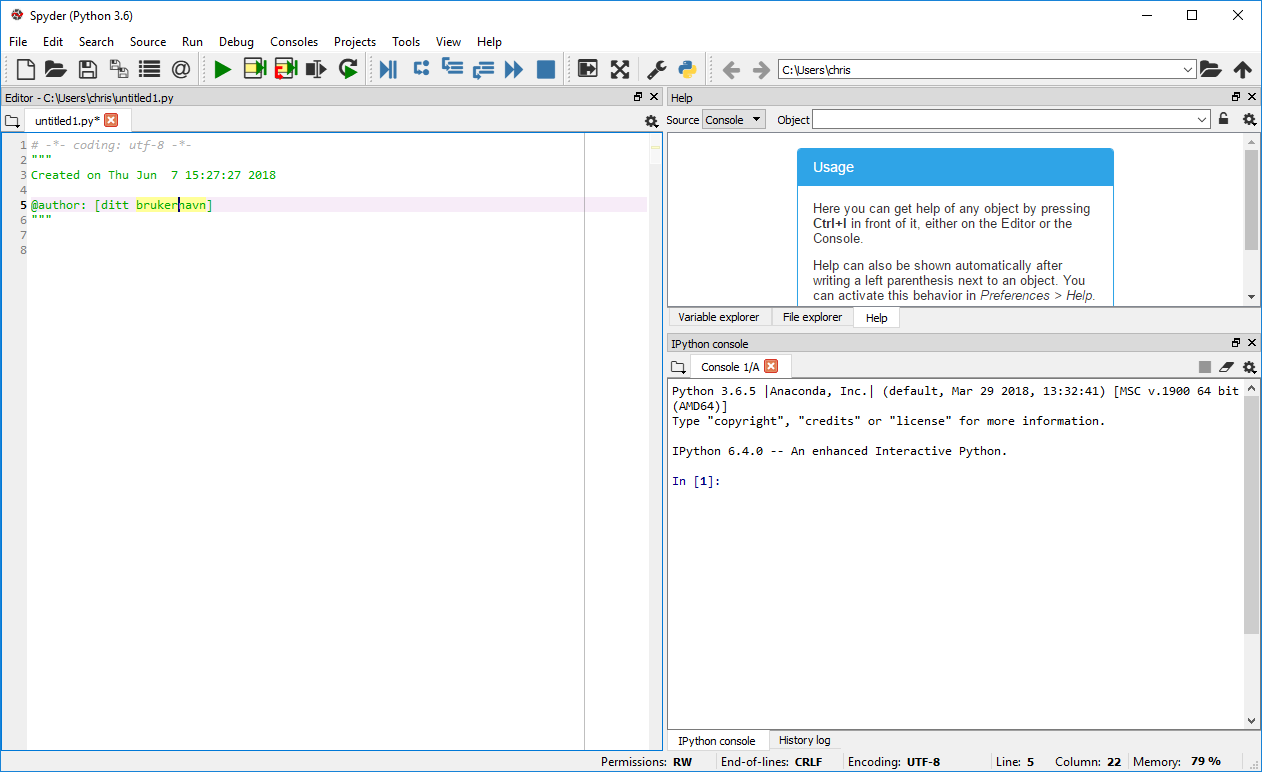
\includegraphics[width=1.0\textwidth]{img/spyder_overview.png}
\end{center}
\caption{Spyder}
\label{fig:spyder_overview}
\end{figure}

Start Spyder. Du skal da på skjermen ha et stort vindu, typisk med tittel Spyder (Python 3.6) Helt øverst er den vanlige menylinjen ( \menuitem{File} \menuitem{edit} \menuitem{search} \ldots..). Like under er der en linje med forskjellige ikoner. Dette er ulike toolbars. De er snarveier til funksjonaliteter som også kan nås fra menylinjen. Toolbarene kan flyttes rundt eller fjernes helt ved \menuitem{View} \menuitem{Toolbars} og klikke de av.) Vi trenger ikke tenke på disse ennå. 

Under linjen med toolbars, på venstreside har du Editor-vinduet. Det er et tekstbehandlingsprogram.  Her er det du skriver inn Python programmet ditt, linje for linje. Du kan flytte deg rundt med piltastene (og musen). Ikke skriv noe ennå. 

Hvis dette er første gangen du bruker Spyder, vil Spyder ha lagt inn noe tekst i et nytt dokument. På linje 5 eller 6 vil det stå @author og brukernavnet ditt. Navnet på filen står øverst, noe slikt som \emph{untitled1.py}. Dette er en fil som Spyder har åpnet og som ikke gjør noe ennå. Hvis du allerede har brukt Spyder litt, vil kanskje den siste fil/programmet du arbeidet med være i editoren.

Når programmet (det du har skrevet inn) er klart, kjører (eksekverer, execute) du det ved å trykke på den grønne \emph{play}-knappen, like under menylinja øverst. (Den viser \emph{Run file (F5)} når du holder musepekeren over knappen). Ikke gjør det nå. Vi skal ikke bruke editoren nå helt i begynnelsen.

På høyresiden, nederst, har du Python/IPython-vinduet, også kalt konsollen (Console). Nederst står det \tabitem{Python console}, \tabitem{IPython console} og/eller \tabitem{History log} avhengig av hvilken versjon du kjører. Klikk på tab-en \tabitem{IPython console}. Du kan også bruke Python console, men IPython er å foretrekke. I IPython-vinduet kan du skrive Python kommandoer direkte inn. Det skal vi gjøre mye av nå i begynnelsen. (I'en i IPython står for interaktivt, dvs. to-veis kommunikasjon mellom deg og Python.) 

På høyresiden, over IPython-konsollen er der et vindu. Dette har tab-ene \tabitem{Help}, \tabitem{Variable explorer} og \tabitem{File explorer}. Litt mer om det nedenfor. 

Python har mange kommandoer (funksjoner) innebygd. Det er disse vi bruker når vi programmerer. Den første funksjonen vi trenger er print (skriv til skjerm), Klikk på (inne i) IPython-vinduet for å aktivere det. Skriv så første linja nedenfor og trykk \keypress{enter} :
\begin{lstlisting}
print(365)
\end{lstlisting}
Python skriver ut \verb|365|.

Prøv:
\begin{lstlisting}
print("Hei Python")
\end{lstlisting}

(Merk at tekst må stå innenfor hermetegn)

print() er en funksjon, og funksjoner tar argumenter i parentes. Argumentet til print er det som skal printes, her tekststrengen ``Hei Python'' eller tallet \verb|365|.

\subsubsection{Variabler}
En variabel er noe som inneholder en verdi. En variabel har både et navn og en verdi.

\begin{lstlisting}
min_var1 = "Hei Python!"
\end{lstlisting}

Navnet er \lstinline{min_var1}, verdien er ``Hei Python''. Det er en tekststreng (str). 

\begin{lstlisting}
min_var2 = 365
\end{lstlisting}

Navnet er \lstinline{min_var2}, verdien er $365$, det er et (hel)tall (int). 

\begin{lstlisting}
min_var2 = 300
\end{lstlisting}

Nå skiftet vi verdi. 

Du kan godt ha mellomrom, linjene over kan også skrives som: 
\begin{lstlisting}
min_var2=300
min_var2= 300
min_var2 =300
\end{lstlisting}

Men du kan ikke skrive \verb|min var2 = 300| for variabelen heter \lstinline{min_var2}, den må være i ett ord. 

Nå kan vi printe variabelen:
\begin{lstlisting}
print(min_var1)
\end{lstlisting}
Flere variabler og verdier kan printes samtidig:
\begin{lstlisting}
print(min_var1, "Det er", min_var2, "dager i et år.")
\end{lstlisting}

I IPython-vinduet kan du bruke piltastene for å hente frem igjen det du har skrevet tidligere. Prøv pil opp, og ned igjen. Du kan også endre på linja, og trykke {\em enter} for å kjøre/utføre (eksekvere) linja (på nytt). (Eller visk ut linja eller trykk piltast ned til du får tom linje.) Du kan også se alt du har skrevet i vinduet ved å trykke på History log nederst. (Gå tilbake til IPython-vinduet.) 

\subsection{Variable explorer}

Nå har du definert et par variabler (min\_{}var1 og min\_{}var2). I vinduet oppe til høyre, kan du se innholdet til variablene. Klikk på flappen ``Variable explorer''. Det kan være nyttig når du har litt større programmer og programmet ikke helt oppfører seg som du tenkte. (Mer om debugging senere.) 

I IPython-vinduet trenger du forsåvidt ikke bruke print for å se verdien til en variabel, bare skriv navnet og trykk {\em enter}:
\begin{lstlisting}
min_var1
\end{lstlisting}

Det blir ikke helt som med print. Hermetegnene vises. Og det er dessuten enkle hermetegn, og ikke doble som vi brukte. Både doble og enkle hermetegn kan brukes i Python. Men de må stemme parvis. Du kan ikke skrive:

\begin{lstlisting}
min_var3 = 'Hei"
\end{lstlisting}

Da får du en feilmelding: ``SyntaxError''

\subsection{Feilmeldinger}

Når du skriver noe som python ikke forstår, får du en feilmelding.  Lag noen feil og se hva Python svarer:


\begin{lstlisting}
asdf
\end{lstlisting}

Du får \texttt{NameError} - python aner ikke hva \texttt{asdf} skal bety.

\begin{lstlisting}
'asdf'
\end{lstlisting}

Nå er \texttt{asdf} innenfor hermetegn, og da er det bare en verdi. Python klager ikke.

\begin{lstlisting}
a = "asdf
\end{lstlisting}

\texttt{SyntaxError: EOL while scanning string literal}

Du vil komme borti flere feilmeldingerstyper. Det er viktig å skjønne hva feilmeldingen betyr. I interaktiv kjøring, er det alltid siste kommando som er feil, så vi vet hvor feilen er. Når vi kjører et program fra fil, og noe går galt, forteller Python i hvilken linje
feilen oppstod. Det er praktisk. 


\subsection{Tab-completion}

IPython-vinduet ditt kan hjelpe deg med å skrive raskere. F.eks. skriv \lstinline{pri} og trykk {\em tab}. IPython fullfører så med å legge til \lstinline{nt} så det blir \lstinline{print}. Det er den i stand til fordi der kun er én kommando som begynner med \lstinline{pri}. Dersom du bare skriver pr og trykker TAB kommer det opp noen flere alternativer. Du kan velge med piltastene (og {\em enter} eller {\em tab}, eller trykke {\em escape} for å kansellere.

Tab-completion plukker også opp variabler. Dersom du skriver \lstinline{mi} og trykker {\em TAB}, blir en \lstinline{n} lagt til så du har \lstinline{min}, og du får flere alternativ, \lstinline{min} (som er en funksjon som vi skal komme tilbake til),
eller variablene du selv har definert, \lstinline{min_var1}, \lstinline{min_var2} og \lstinline{min_var3}.


\subsection{Spyder}
Restarte IPython-vinduet. Noen ganger henger IPython-vinduet, og du må restarte for å komme videre. Eller du har kanskje lyst til å bli kvitt alle variablene du har definert, starte med blanke ark.  Da kan du trykke på Consoles i hovedmenyen øverst, deretter Restart kernel. Da går det noen sekunder, så kommer et nytt, rent IPython-vindu opp. (NB: du mister altså alle variablene du har laget. Du trenger ikke gjøre det nå.)

Du kan også ha flere IPython- og/eller Python-terminaler oppe samtidig. Klikk Consoles, og deretter Open an IPython console eller Open a Python console.

Restarte Spyder. Dersom du vil ta ned hele Spyder: Se oppe til venstre, trykk File, så Quit. (Ikke gjør det nå.) 


\subsection{Litt mer om Spyder: Layout} 
Spyder er en GUI (Grafisk User Interface, grafisk brukergrensesnitt) som gjør det enklere å arbeide med Python. Spyder eksisterer for windows/mac/linux og er open source og gratis. Vi har installert det som en del av Anaconda eller Miniconda. (Det går naturligvis også an å kjøre Python uten Spyder.)

Spyder har mange funksjonaliteter. (Se de mange valgene i hovedmenyen øverst i vinduet.) En av disse er hvordan layouten skal være. Trykk på View / Window layouts. Sansynligvis er det Spyder Default Layout du bruker. Du kan velge en av de andre, f.eks. Matlab Layout. Den gir deg flere vinduer med informasjon, som kan være nyttig. Men vi holder oss til Spyder Default Layout.

Du kan justere størrelsen på vinduene med musen.

Du kan øke/minske tekststørrelsen i Editor-vinduet og IPython-terminal-vinduet (uavhengig av hverandre) med CTRL+ / CTRL- mens vinduet er aktivt. 

Noe som kan være praktisk nå i begynnelsen, er muligheten til å lagre alt som er gjort i IPython-vinduet. Aktiver IPython-vinduet. Trykk så CTRL+s (CTRL og s). Da kommer et vindu opp som lar deg lagre IPython-aktiviteten som html-fil. Velg et passende navn (og katalog). Filen må leses med en nettleser (Firefox, IE/Edge, Safari). (Enten kan du finne filen med f.eks. Windows Explorer, dernest klikke på den. Eller du kan åpne en ny tab/vindu i nettleseren og skrive file:/// i url-en. Da vil du få opp filstrukturen din. Du må da klikke deg frem til rett sted og finne filen.) Det går imidlertid ikke an å laste det inn igjen i spyder og slik fortsette der du slapp. 

\section{Oppgaver}

\begin{question}
Bruk et minutt eller to på å gjøre deg litt kjent med Spyder. Endre litt på vindusstørrelse, klikke på ulike flapper, sjekke hva menyene inneholder.
\end{question}
\begin{question}
Lag to variabler som inneholder tall. Lag to variabler som inneholder tekst. Skriv ut innholdet av de fire variablene. Se om de er i Variable explorer-vinduet. Endre innholdet til en av variablene. Se om variabelverdien endres i Variable explorer.
\end{question}
\begin{question}
Lagre en html-fil med IPython-aktiviteten din og finn den igjen med en nettleser.
\end{question}

REF: For mer Spyder-info: klikk på Help-flappen på vinduet øverst til høyre (som også har flappen Variable explorer). Der kan du ved anledning (senere) følge en tutorial (klikk tutorial) som beskriver ganske greit hva Spyder har å tilby.

\iffalse

######################################################################## 
KAP. 2.2  TALL

TALL, MATEMATIKK
Operasjoner: + - * / ** parenteser

Prøv følgende:
(NB: Python leser ikke det som står til høyre for # på en linje.
Det kaller vi en kommentar, så den delen trenger du ikke skrive, bare mattestykket.)
(Du kan også ha en hel linje som starter med #, en kommentarlinje.) 

# Dette er en kommentar. Her kan jeg skrive noe stygt som Python ikke leser ... (Python er et dårlig språk) 
2+2   # pluss, addisjon
4-2   # minus, subraksjon
2*3   # gange, multiplikasjon
7/3   # dele, divisjon
2**3  # opphøyd i, dette er 2*2*2

Maskinen regner ikke fra venstre mot høyre. 
Den har regler for hva som skal regnes ut først: 
Prioritert rekkefølge: først ** så * og /, så + og -. 
4+3*2   # 14 eller 10? 
3*2**2  # 36 eller 12?

Men hva gjør vi om det faktisk er slik at vi vil at 4+3 skal regnest ut først,
så skal vi gange resultatet med 2? 
Da bruker vi parenteser. Parenteser har enda høyere prioritet enn **,
dvs. det som er inni en parentes blir alltid regnet ut først.
Så, vil vi regne ut 4+3 først, gjør vi det slik: 
(4+3)*2 
Er det forskjell på 4+(3*2) og 4+3*2? 

Disse prioriteringsreglene er de samme som på kalkulatoren din. 

Du kan ha mellomrom (space) hvor som helst mellom de ulike elementene på en linje,
de spiller ingen rolle. 
4 + 3*2
4+3 * 2 
Men første tegn er hellig, det må stå der det skal stå 
Linja under vil derfor gi feilmelding siden linja starter med en space (IndentationError). 
 4+3*2

Men: Når du skriver det direkte inn i IPython-konsollen, får du (dessverre) ikke
feilmelding i linja over.
IPython-konsollen forstår hva som er ment.
Python-konsollen vil imidlertid gi feilmelding.
Prøv. (Du må da klikke på Python console nederst. Og etterpå tilbake til IPython.) 
Og hvis du gjør det i et program, som er det vi vanligvis vil gjøre, får du også feilmelding. 

Du kan naturligvis heller ikke sette et mellomrom midt i et tall,
f.eks. skrive 44 + 3 som 4 4 + 3). 



Vi bruker de matematiske operasjonene til å regne ut ting og tang.
Vanligvis gjør vi det slik:
EN VARIABEL = ET REGNESTYKKE
Dette er metakode, dvs. ikke virkelig kode, men kode-aktig. 
Den vil ikke fungere om du skriver den inn i IPython-konsollen.
Mer standardisert måte er å omslutte forklaringene i vinkelparenteser.
<en variabel> = <et regnestykke> 
(Den fungerer fortsatt ikke i IPython-konsollen.)
Det som er omsluttet skal erstattes av syntaktisk korrekt kode.
Du vil ofte møte slik kode, f.eks. når du leter på nettet.


Eksempel (på matematikk, ikke på metakode)
a = 5 + 3
Her blir variabelen a, som er på venstresiden, satt til å være lik 5 + 3, altså 8. 
(Det kan du se ved å bare skrive a, eller print(a). Du ser det også i Variable explorer.) 
Dette kalles tilordning (assignment), a blir tilordnet verdi 8.
Der er litt ulike meninger om man bør ha mellomrom mellom tallene og tegnene.
Der finnes visse stil-standarder. Litt mer om style senere. 

Ofte er det ikke bare tall som står på høyresiden, men også andre variabler. 
b = 2*a + 3  # Her får variabelen b verdien 2*8 + 3 = 19  (fordi a = 8, se ovenfor).
Hvis a ikke er definert, vil du få feilmelding. 
Prøv i stedet: 
b = 2*c + 3 
Da klager python (rettmessig) over at c ikke er definert. 

Det er også mulig at den variabelen som står på venstresiden også står på høyresiden.
a = 2*a + 3
Men hvordan skal det forstås? Hvordan forstår python det? 
Regelen er at høyresiden regnes ut først, så blir venstresiden,
som alltid må være en variabel, satt lik denne verdien. 
Variablen a blir altså her 19 til slutt.
(a'en på høyresida er 8, men når linja er ferdig utført, har a fått verdi 19.)  
Linjen ovenfor skal altså IKKE leses som en ligning.
Den matematiske ligningen a = 2a + 3 har løsning a = -3.
Og det er ikke det som skjer i denne linja. 
Det kan virke merkelig å bruke samme variabel på høyre og venstre side.
Men det er ofte brukt. 

Kan vi skrive følgende ligning? 
x + 5*3 = 3
(Nei. Prøv. Det gir SyntaxError.) 
Har vi en variabel som er definert gjennom en ligning,
og vi vil at Python skal regne ut denne variablen,
da må vi først løse ligningen (på ark) slik at vi får variabelen alene på venstresiden.
For ligningen ovenfor blir det slik: 
x = 3 - 5*3
NB: Der finnes en pakke (package) i python som løser ligninger for oss: sympy. 
Den kan regne algebraisk, symbolsk. 
Da slipper vi å løse ligningen selv.
Vi skal se på sympy senere. 


I oppgavene nedenfor: regn ut for hånd (kalkulator). Prøv så i python. 

Oppgave 1:
Hva blir 2*3-4/2*2, (1-3)*(-3)/(2*2), 2*3**2/2, 1/2**3-4-8/2*4 , 2**3-(4-8)/2*4 ?  

Oppgave 2:
Regn ut arealet av en firkant med side a=3 og b=12. (Diskuter med sidemannen.) 

Oppgave 3: Regn ut omkretsen av en firkant med side a=4 og b=5.

Oppgave 4: Løs 3x - 2 = 13 

Oppgave 5: Regn ut omkretsen av en sirkel med radius 3.
(Hva er radius? Og pi? Diskuter med sidemannen.) 

######################################################################## 
KAP. 2.3  DATATYPER #1: int, float, str

Verdien til en variabel er alltid av en viss type,
f.eks. en tekststreng eller et heltall eller et desimaltall. 
Typen avgjør hva vi kan gjøre med variabelen.
For eksempel kan to tall multipliseres (ganges) med hverandre.
3.3*4.1
Men det gir ikke mening å gange to tekststrenger med hverandre.
'asdf' * 'abc'
Da klager python.
(Men det gir faktisk mening å skrive 3 * 'abc'. Prøv.) 

Funksjonen type() forteller oss hvilken datatype en variabel (eller en verdi) har. 
Prøv: 
type(23)               # int    (integer, heltall) 
type(23.3)             # float  (desimaltall) 
type(23.0)             # float  
type('23')             # str    (tekststreng) 
a = 43.3
type(a)

Merk at vi for desimaltall bruker punktum, ikke komma.
(Det er engelskspråklig stil, som er den som er brukt i programmering.) 
NB: vanligvis vil argumentet ikke være et tall, men en variabel, f.eks. type(min_var). 

Noen ganger er det viktig å skille mellom int og float, men som oftest ikke. 
(I tidligere versjoner av Python, er det veldig viktig å skille mellom int og float.
I Python2 vil 1/2 ikke gi 0.5, men 0 fordi det er såkalt heltallsdivisjon. 
Vi kjører Python3, nærmere bestemt Python 3.6) 


Omgjøring av datatyper (recast): 

Fra tall til tekst: 
str(33.0)        # gir '33.0'
str(33)          # gir '33'
type(str(33))    # str
a = 334
str(a)
type(str(a))     # str

Fra tekst til tall: 
int('345')       # gir 345
float('345')     # gir 345.0  (float) 
float('345.3')   # gir 345.3 
int('345.3')     # gir feilmelding

Fra int til float: 
float(33)        # gir 33.0

Fra float til int 
int(33.3)        # gir 33
int(33.6)        # gir 33 (!) 
int() runder altså ikke av slik vi er vant til, den bare fjerner desmaldelen. 


Der er en annen funksjon som runder av, round(). 
round(33.5)      # blir 34 
round(33.499)    # blir 33
Med round kan du også runde av til et gitt antall desimaler (default er null desimaler).
round(33.499,2)  # blir 33.50
round(33.43,1)   # blir 33.4

(NB: vanligvis er det variabler vi har som argumenter, ikke verdiene selv.)  




Oppgave 1: Du har to tekstvariabler, a = ' 7.3' og b = '30.1'.
Bruk korrekt omgjøring av datatyper og finn så differansen (den ene minus den andre),
summen og produktet (den ene ganget med den andre). 

Oppgave 2: Du har c = '7.345'.
Er det mulig å runde av tallet til to desimaler på bare en linje?

Oppgave 3: Du har en variabel a = 3.14 og b = "Pi er ".
Lag en tekststreng c som kombinerer a og b og gir verdien "Pi er 3.14". 

######################################################################## 
KAP. 2.4  IMPORTERE PAKKER

Python har en del innebygde (builtin) funksjoner.
Disse er tilgjengelig idet vi starter opp Python.
F.eks. alt vi har nevnt så langt: print(), int(), float(), str(), type(), round()
Noen flere som kan være nyttige for oss: abs(), max(), min() 

Prøv: 
abs(-3)          # tar absoluttverdien (dvs. fjerner eventuelt minus foran)
abs(-3.3)
max(1,3,99,-29)  # finner maksimumsverdi av en liste med tall
min(1,3,99,-29)  # finner minimumsverdi 


Men mye mye mer er tilgjengelig som pakker (packages) som vi kan laste inn etter behov.
F.eks. finnes der en pakke som heter math.
Der finnes blant annet pi (3.14159...) og kvadratrot (sqrt) og sinus (sin). 
For å bruke det som finnes i pakken, må vi først importere den. 
import math
Da kan vi gjøre f.eks.
math.pi 
For å se hva som finnes i math, kan vi skrive math. (math og punktum), trykk så TAB.
Da kommer det opp en liste over funksjoner (og f.eks. konstanter som pi), bl.a. math.sin()
Prøv
math.sqrt(9)         # Kvadratroten (square root, sqrt)
math.sqrt(2)         # 
math.sin(1.57)       # Skal bli nesten 1
math.sin(math.pi/2)  # Skal bli akkurat 1

NB: De trigonometriske funksjonene (sin, cos, ...) tar argumentet i radianer,
ikke i grader. 
Har du vinkelen i grader, må du først regne om til radianer.
180 grader tilsvarer pi (radianer). (pi er 3.14159265...) 
Så har du g grader tilsvarer det r = pi * g / 180  radianer.
(Og har du r radianer, tilsvarer det g = 180 * r / pi  grader.) 

Der er også funksjoner som gjør akkurat disse omregningene: 
math.radians() og math.degrees()
Prøv. 

Der finnes et knippe forskjellige måter å importere en pakke på.
Du vil sannsynligvis møte alle metodene når du leser andre sin kode,
så greit å ha sett dem. 
Du vil sannsynligvis bruke flere av metodene selv.

Metode 1: (den vi hadde ovenfor)
import math
print(math.pi)
Du må ha math. foran funksjoner/konstanter fra pakken

Metode 2:
import math as ma
print(ma.pi)
Som første metoden, men pakken blir hetende ma i stedet for math.

Metode 3:
from math import pi,sin, sqrt
print(pi)
I dette tilfellet importerer du kun pi, sin og sqrt fra pakken.
Du slipper å ha math. foran. 

Metode 4:
from math import *
print(pi)
Som ovenfor, du slipper å ha math. foran.
Men du importerer alle funksjonene i pakken. 
Det unødvendig, og generelt ikke anbefalt.
(Faren er at pakken (her math) kan ha en variabel eller funksjon med samme navn
som noe du har definert tidligere, og vil da erstatte denne.) 
(For små programmer er det imidlertid faren kontrollerbar.) 


Pakken math er del av det såkalte Python Standard Library
(https://docs.python.org/3/library/)
Vi skal bruke noen av pakkene der.
Bl.a. pakken random
Denne bruker du til å velge tilfeldige tall.
Den er nyttig f.eks. i spill. Vi skal bruke den om litt. 
import random
random.random()          # gir et tilfeldig desimaltall mellom 0 og 1
random.uniform(7,17)     # gir et tilfeldig desimaltall mellom 7 og 17
random.randint(1,6)      # gir et tilfeldig heltall mellom 1 og 6. (Grensene, altså 1 og 6, er valgbare.) 


Hvis du har importert math i alle mulige fasonger (ovenfor),
kan det være på sin plass å restarte IPython-konsollen (CTRL+.)
før du begynner på oppgavene nedenfor. 


Oppgave 1: En rett vinkel er 90 grader. Finn sin og cos til en rett vinkel.

Oppgave 2: Finn et tilfeldig desimaltall mellom 0 og 1, mellom -5 og 5, mellom -2 og 18.

Oppgave 3: Finn et tilfeldig heltall mellom 0 og 9, mellom -5 og 5, mellom -2 og 18.
Grensene skal være med. 

Oppgave 4: Finn cos og sin til 35 grader.
Regn også ut kvadratet av sin og av cos, og ta summen.

Oppgave 5: Finn cos og sin til 2.3 radianer 

Oppgave 6: Finn kvadratroten av 256. 

######################################################################## 
KAP. 2.5  NY FUNKSJON: input : lese fra tastaturet 

Få opplysninger fra brukeren ved funksjonen input()
navn = input("Hva heter du? ") 
print("Du heter", navn)
input() leser inn en tekststreng. 
Selv om du skriver et tall, vil input gi en tekststreng. 
alder = input("Hvor gammel er du? ")   # svar med et tall 
print(alder)
type(alder)
Type avslører at det er en tekststreng.
Derfor kan du ikkje gjøre følgende
print(alder + 13)
Feilmelding (TypeError), du ikke kan legge sammen et tall og en tekst. 

Hvis det er et tall du ønsker å lese inn (alder), må du selv gjøre om til tall. 
alder = int(alder)
(Evt. kunne du brukt alder = float(alder).)
Nå har du gjort om alder til heltall.
Da fungerer dette fint: 
print("Om", 13, "år er du", alder+13, "år") 
NB: dersom du bruker int(alder), men oppgir f.eks. '21.5', vil du få feilmelding. 


Oppgave 1: Be om et tall med input(). Gjør den innleste verdien om til float,
og finn til slutt kvadratroten og multipliser med pi. 

######################################################################## 
KAP. 2.6  LAGE ET PROGRAM, EN FIL

La oss nå lage et program, dvs. opprette en fil og kjøre (eksekvere) den. 
Klikk på vinduet til venstre, editoren. 

Dersom du ikke har lastet inn en fil, vil editoren inneholde følgende tekst (omtrent): 

# -*- coding: utf-8 -*-
"""
Created on Sun Aug  6 18:49:51 2017

@author: nobody
"""

Dersom du har et annet program (en annen fil) inne i editoren,
kan du begynne på en ny fil ved å trykke på File, så New file.
Programmet/filen vil da bli hetende noe sånt som untitled0.py inntil videre,
til du med File / Save as gir den et bedre navn. 

Legg inn følgende tekst under det som allerede finnes, dvs. ca. fra linje 7: 

navn = input("Hva heter du? ")
alder = input("Hvor gammel er du? ") 
print("Du heter", navn, "og er", alder, "år gammel.") 

Trykk så File fra menyen øverst, dernest Save as. 
Du bør nå velge en grei plass på maskinen for python-filer. 
Du kan også lage en folder her og nå med New Folder og klikke deg inn i den. 
Filnavnet bør være beskrivende, f.eks. tut_prog_navnogalder1.py. 
Filen må ha ending ".py". 
I Windows blir .py lagt til automatisk dersom du ikke selv gjør det. 


For å kjøre filen, trykker du på den grønne pilen øverst til venstre (Run file),
eller trykker F5. 
I det interaktive vinduet (IPython-konsollen) får du nå spørsmål å svare på. 
Du må sannsynligvis først aktivere vinduet ved å klikke på det
før du kan skrive inn navn (og trykke ENTER) og alder (og trykke ENTER). 
Merk at mens programmet kjøres, kan du ikke bruke IPython-konsollen til andre ting
(f.eks. til å regne ut 365+366). 
Når du har oppgitt navn og alder avsluttes programmet.
Da kan du igjen bruke det interaktive vinduet til andre ting. 

Du kan kjøre programmet på nytt ved igjen å klikke på den grønne pilen.

Dersom du gjør endringer i programmet, kan du lagre endringene ved å
klikke File / Save (eller trykke CTRL+s). 
Eventuelle endringer som ikke allerede er lagret, vil bli det hvis du trykker på
den grønne filen og kjører programmet.


Det er viktig å bli komfortabel med filer, vite hvor de er, kunne lagre,
kunne opprette nye, laste inn filer du har laget tidligere etc.
Vanlig bruk av python er via filer. 
Kun for veldig små oppgaver vil du skrive kommandoene direkte inn i IPython-konsollen. 
I linjen over editor-vinduet, vil der vere en eller flere flapper,
og kanskje piler til venstre/høyre.
Dette er aktive filer. Du kan klikke på en flapp, så blir filen lastet inn i editoren.
Dersom du har andre python-programmer tilgjengelig på harddisken,
kan du laste inn disse ved å klikke File / Open, og så finne frem til den aktuelle filen. 



Oppgave 1:
Lag et program som leser inn fornavn, etternavn og alder i passende variabler.
Omtrentlig fødselsår skal så regnes ut, og når du fyller 50 år.
Skriv til slutt ut alle opplysningene. 

Oppgave 2:
Lag et program som leser inn navnet ditt, og så finner et tilfeldig tall
mellom 15 og 35, og påstår at det er alderen din.

######################################################################## 
KAP. 2.7  BETINGELSER 

Ofte må man i et programmet gjøre forskjellige ting avhengig av verdien til variablene. 
I python gjøres dette med if-konstruksjonen 
Skriv in følgende programsnutt i et nytt dokument og kjør det: 

alder = 18
if alder < 20:            # merk kolonet og indenteringen nedenfor
   print("Tenåring")      # Dette blir utført hvis alder er mindre 20
   print("fortsatt")      # også dette, siden det også er indentert
print("Dette blir printet uansett")

Her er å merke seg at to linjer er forskyvd mot høyre, de er indenterte.
Det som er indentert blir utført dersom alder < 20. 
Siste linja er det ikke indentert. Det blir printet uansett alder.

Det er altså via indenteringen du forteller Python logikken i if-setningen din.
Editoren du bruker (spyder, emacs, ..) kjenner til indenteringsreglene i python.
Det vil derfor typisk foreslå indentering når du trykker ENTER etter kolonet.
Når du er ferdig med indenteringen, må du selv avslutte den ved å trykke
BACKSPACE eller SHIFT+TAB. 

Prøv å skrive inn manuelt (ikke copy/paste), se om Spyder oppfører seg slik den skal. 

(NB: hvis du av en eller annen grunn ikke har .py som endelse på filen,
vil editoren ikke nødvendigvis vite at du skriver i python,
og da heller ikke hjelpe deg med indenteringen.) 


Mer komplisert if-setning: 
En if-setning kan også inneholde else, som betyr otherwise/hvis ikke.
Dette utføres dersom if-betingelsen ikke er tilfredsstilt. 

if alder < 20: 
   print("Tenåring")
   # gjerne flere linjer
else: 
   print("Olding")     # Dette utføres dersom alder ikke er < 20
   # gjerne flere linjer

Du kan også teste flere alderskategorier (elif, som forstås som else if) 

if alder < 20: 
   print("Tenåring")
elif alder < 30:           
   print("Olding")         # mellom 20 og 30 (hvorfor?) 
elif alder < 40: 
   print("Nesten ferdig")  # mellom 30 og 40 (hvorfor?)
else: 
   print("Ung igjen")  # 40 eller mer 

Merk logikken.
Vær sikker på at du forstår hvorfor alderen må være mellom 30 og 40
på tredje siste linje.
(Poenget er at hvis vi allerede har kommet til elif alder < 40, vil vi allerede
ha feilet på alder < 30, dvs. alderen er 30 eller mer.) 


Mer generelt ser konstruksjonen slik ut

if <BETINGELSE1>: 
   <handling1>
elif <BETINGELSE2>: 
   <handling2>
<evt. flere elif-bokkker>
else: 
   <handling_resten>


Handling kan gå over flere linjer. 


Verdien til BETINGELSE er True eller False.
(NB: stor førstebokstav, resten små. Verdien er ikke true eller TRUE, men True.)
Dette er en ny datatype: logisk (boolsk, boolean).
En boolsk variabel (eller uttrykk) har altså kun to mulige verdier: True eller False. 

Ofte blir den produsert via følgende sammenligningsoperatorer 
 <  : mindre enn
 >  : større enn
 == : er lik  (NB: ved sammenligning bruker vi == ikke =)
 <= : mindre enn eller lik
 >= : større enn eller lik 
 != : ikke lik


Prøv (interaktivt, dvs i IPython-konsollen): 
2 == 3   # False
2 = 3    # Dette må vel gi feilmelding? (Tilordning/assignment)
2 == 2   # True
2 != 2   # False
2 != 3   # True
2 < 3    # True
2 > 3    # False
2 <= 2   # True
2 >= 2   # True
2 =< 2   # SyntaxError
2 => 2   # SyntaxError

også:
a = 2    # tilordning
a == 3   # sammenligning

navn = "Newton"       # tilordning
navn == "Einstein"    # False 
navn == "Newton"      # True
navn == "Newton "     # False
type(navn)

Du kan også legge resultatet av en sammenligning inn i en variabel:
bet1 = (2 == 3)   
print(bet1)
type(bet1)   # bool


KOMBINERE BETINGELSER: and, or, not 
interaktivt: 
a=2             # (tilordning)
a==1 or a==2    # True 
a>1  or  a<1    # True 
a>1  and a<1    # False
not(3==3)       # False
not(True)       # False  # not snur True til False og False til True
not(False)      # True 



Betingelser og logiske operatorer blir utført i en viss rekkefølge.
Dersom du er usikker på om den rekkefølgen du ønsker faktisk er det Python gjør,
eller om du vil fremheve logikken for den som leser koden, 
kan du alltid sette inn parenteser.



Oppgave 1: Lag et program som leser inn tre tall, gjør de om til float, 
så sjekker hvilket av de tre som er størst og skriver til skjerm om
det var det første, andre eller tredje som ble skrevet inn. 


Oppgave 2: Lag et program som finner et tilfeldig tall mellom 1 og 10
(grenser inkludert), og så ber deg gjette tallet.
Programmet sier til slutt ifrå om du gjettet for høyt, for lavt eller riktig. 


Oppgave 3: Lag et program som simulerer tre terningkast og skriver ut hvor mange
like det ble (3 like, 2 like eller ingen like). 


Oppgave 4: Lag et program plukker to tall, x og y, mellom (f.eks.) 10 og 100. 
Brukeren blir så spurt om å svare på følgende regnestykker, x+y, x-y, x*y (etc?) 
For hvert regnestykke kontrollerer programmet svaret og skriver en kommentar. 

######################################################################## 
KAP. 2.8  NY DATATYPE: LIST
(Nye funksjoner: len, help, range

Datatyper så langt: int, float, str, bool


Datatypen list er en liste (sekvens) med elementer. 
Elementene kan være tall, tekst, andre lister eller andre ting.

Prøv i IPython-konsollen:

liste1 = [1,3,5,2,33,0,2]  # deklarerer og fyller en liste med tall
type(liste1)

(Du trenger å bruke hakeparentesene. 
Med engelsk tastatur (som ofte er det enkleste for programmering), 
er de lette å nå. Med norsk tastatur er det via alt gr. (Mac: alt)) 

en_liste = []        # tom liste
en_liste2 = list()   # kan også lage tom liste slik

hummer = [32,'Toyota',333]   # elementene trenger ikke være av samme datatype

biler = ['Toyota','Mazda','Audi'] 
len(biler) 

len() (length) er en funksjon som viser antall elementer i en liste. 


help() er en annen funksjon. Den viser info om det du putter inni parentesen, 
f.eks. en funksjon
help(len)
help(print)
help(list)
(Når du putter inn en variabel, får du info om den typen det er. 
help(biler) vil vise så å si det samme som help(list).)  
Beskrivelsen i help kan være ganske teknisk. 
Det er ikke alltid så lett å finne frem til det man leter etter.
Ofte er et søk på nettet raskeste vei, men help() kan også være til god hjelp. 


Tilbake til lister. 
Vi kan aksessere (rekke, nå) elementer i listen ved å angi indeksen til elementet. 
I Python (som i bl.a. C) starter en liste med indeks 0.
(Det kan være forvirrende i begynnelsen.) 

biler[0]       # den første bilen 
biler[1]       # den andre bilen
biler[2]       # den tredje (og siste) bilen
biler[3]       # IndexError
biler[len(biler)-1]   # den siste bilen (fordi vi starter på 0) 
biler[-1]      # triks. den siste bilen, faktisk. 
biler[-2]      # triks. nest siste bilen. 
biler[-3]      # triks. tredje siste bilen (som er det første)
biler[-4]      # IndexError igjen


Hvilke funksjoner (metoder) eksisterer for en liste?
Skriv biler. og trykk TAB. 
Du får opp funksjoner som append, clear, count, ... 
La oss se på noen av dem. 


Legge element bakerst i listen / Legge til elementer: 
biler.append("Tesla")
print(biler)

Legge Mercedes inn som bil nr. 3 og skyve Audi og Tesla til bil 4 og 5 
biler.insert(2,'Mercedes')
print(biler)

Kan erstatte elementer
biler[1] = "Golf"
print(biler)

Du kan også legge til elementer på følgende måte:
biler = biler + ['Honda','Renault']
og/eller 
biler = ['BMW','Volvo'] + biler


Du kan aksessere (velge) en del (en slice) av listen ved å spesifisere to indekser.
Prøv: 
print(biler)
biler[2:5]
De to indeksene er det første elementet du vil ha med,
og til det siste elementet du vil ha med PLUSS 1. 
biler[2:5] viser element 2, 3 og 4, som er bil 3, 4 og 5. 
Det kan være forvirrende. 

biler2 = biler[2:5] 
print(biler2)
print(biler)          # NB: biler endres ikke 

Prøv også: 
biler[1:1]   # tomt
biler[1:2]   # element 1


Du kan også droppe første eller andre indeks.
biler[:5]     # viser de 5 første bilene
biler[2:]     # viser fra bil nummer 3 og til enden av listen
biler[-3:]    # viser de tre siste bilene


Hvilke flere funksjoner finnes for lister?
skriv biler. og trykk TAB, da ser du funksjoner. 
F.eks.:

biler.sort()          # sorterer listen. Her: alfabetisk sortering
print(biler)

biler.reverse()       # reverserer listen. 
print(biler)

NB: .sort() og .reverse() endrer listen. 

biler.index('Tesla')  # angir hvilket nummer (indeks) i listen 'Tesla' har 
biler.index('Fiat')   # ValueError: 'Fiat' er ikke i listen vår 

biler.pop()           # fjerner siste element fra listen
print(biler)


Du kan også "plukke opp" det som fjernes:
bil1 = biler.pop()
print(bil1)
print(biler)

biler.pop(2)          # fjerner tredje element 

biler.remove('Golf')  # fjerner 'Golf'
biler.remove('Fiat')  # ValueError

Teste om en gitt verdi er i listen vår:
'Fiat' in biler       # False
'Toyota' in biler     # True

F.eks.:
if 'Fiat' in biler:
   print('Ja, har Fiat.')






RANGE()

En litt spesiell måte å lage en liste på er via range-funksjonen
range(5)        # lager listen [0,1,2,3,4]  
range(2,6)      # lager listen [2,3,4,5]
range(2,13,3)   # lager listen [2,5,8,11]

Forklaring: 
Når bare ett argument er gitt, gir det maks-grensen på listen, mens start er 0.
Merk at maks-grensen selv er ikke med i listen.

Når to argumenter er gitt, er det startverdi og maks-grensen.
Igjen: maks-grensen er ikke med i listen. 

Når tre argumenter er gitt, er det startverdi, maks-grensen, dernest hvor mange
steg man hopper mellom hvert element.
Default steg(lengde) er 1, da hopper man ikke over noe, men tar med alle.
Det er det som skjer i de to første range-kallene. 

Sjekk også 
help(range)
(se øverst) 



range() fungerer bare med heltall (int).
(Senere skal vi introdusere arange(), som også fungerer med desimaltall (float).) 


Detalj 1: Merk at range(2,1,3), range(2,14,3), range(2,14,3) gir samme liste. 
list(range(2,12,3))
list(range(2,13,3))
list(range(2,14,3))


Detalj 2: Det er ikke helt sant at range er en liste.
Det ser du dersom du skriver f.eks. range(5) eller print(range(5)).
Hvis det var en liste, ville [0,1,2,3,4] blitt printet. 
Men for de fleste hensyn oppfører det seg som en liste. 
Du kan lage den tilsvarende listen slik:
list(range(5))


Vi bruker ofte range-funksjonen i for-løkker (nedenfor). 




Oppgave 1: Lag et program som leser inn tre navn og legger de i en liste,
sorterer listen alfabetisk og skriver den sortert ut til skjerm, navn for navn. 


Oppgave 2: Som ovenfor, men nå skal det sorteres motsatt vei. 


Oppgave 3: Lag ved hjelp av range() følgende lister:
[0,1,2,3,4,5,6,7,8,9], [0,2,4,6], [2,4,6], [5,8,11,14,17] 


Oppgave 4: Fjern element med indeks 3 fra listen lst1 = [0,1,2,3,4,5].
Fjern så elementet med verdi 2.
Stikk så inn i listen et element 5 slik at det får indeks 2.
Still så inn i listen et element 'fire' slik at det får indeks 2.
Finn så hvilken indeks elementet 5 har.
(NB: du har to like elementer i listen. Forstå hva funksjonen returnerer.)
Fjern så elementet 5 fra listen.
(Igjen, du har to elementer med verdi 5. Se hvilken som fjernes.) 


Oppgave 5: Du har lst2 = [11,22,33,44,55,66,77]
Lag en ny liste som inneholder de tre midterste elementene.
(Det kan gjøres på mange måter. Hva er den raskeste?)

######################################################################## 
KAP. 2.9  FOR-LØKKE (FOR LOOP)

Du vil lage et program som kaster en terning 100 ganger.
Du vil så telle antall ganger du får 5 eller 6. 
Et terningkast kan du simulere med følgende 
import random
tall = random.randint(1,6)   # velger mellom 1 og 6

Men dette skal du gjøre 100 ganger.
Det er ikke spesielt praktisk å skrive opp linjen 100 ganger.
Det er her en for-løkke kommer inn. 

La oss først ta en veldig enkel for-løkke:
(Du kan skrive dette i IPython-konsollen.) 
for i in [0,1,2,3]:
    print(i)
Når du er trykker ENTER etter kolon på første linje,
vil IPython-konsollen selv sørge for å indentere teksten.
Skriv så inn print(i) og trykk ENTER, og ENTER igjen på den tomme linjen etterpå.
Da utføres for-loopen.
(Vanligvis vil vi ha for-looper inne i et program, ikke interaktivt.) 

Hvordan virker en for-løkke?
Iterasjonsvariabelen i går gjennom listen [0,1,2,3]. 
Første gangen er i lik 0, neste gang er i lik 1 etc.
For hver i-verdi blir det som er indentert utført (her kun print(i)).
Det skjer altså 4 ganger her. 

Vi kunne også skrevet listen v.h.a. range(), som altså er nesten det samme som en liste. 
for i in range(4): 
    print(i) 
Det er praktisk dersom du f.eks. skal gjøre det hundre ganger.
Da slipper du å eksplisitt skrive opp [0,1,2,....,99]


Nå er vi i stand til å utføre den lille terningtesten. 

Åpne en ny fil, dvs klikk på ikonet oppe til venstre. (Eller velg File / Open.)
Skriv inn følgende (etter de første 6-7 linjene som automatisk kommer opp): 

import random

# initialisering
n6 = 0  # antall seksere
n5 = 0  # antall femmere

# Løkka 
for kast in range(100):
    tall = random.randint(1,6)
    print("Kast nr", kast+1, "ble", tall)
    if tall == 6:
       n6 = n6 + 1    # øker antall seksere med 1
    elif tall == 5:
       n5 = n5 + 1    # øker antall femmmer med 1

print("Det ble totalt", n6, "seksere og", n5, "femmere.")


Linjer som starter med # er kommentarlinjer. 
Python bryr seg ikke om disse. 

Trykk på grønn pil for å kjøre programmet.
Du får nå beskjed om å lagre filen. Bruk helst samme katalog som sist.
Velg et passende navn, f.eks. tut_for_terning1.py

Hvor mange seksere ble det?
Kjør en gang til.

Med for-loop på reportoaret, er det plutselig mange flere ting vi kan gjøre. 



Oppgave 1: Hva om du brukte range(1,101) i for-linja. Hva ville endret seg?
(Noen ganger bruker du tellevariabelen (iterasjonsvariabelen) inne i løkka,
andre ganger er den ikke i bruk til annet enn å telle f.eks. 100 ganger.) 


Oppgave 2: Tell også opp antall ganger terningen ga 1, 2, 3 og 4, og skriv ut.
Forsikre deg også om at det hele summerer til 100, skriv evt. ut feilmelding. 


Oppgave 3: Som ovenfor, men i stedet for å bruke variablene n1, n2, ..., n6,
bruk heller en liste antall som er initialisert slik: antall = [0,0,0,0,0,0].
NB: antall[0] vil da typisk innholde antall 1'ere. 
NB: Kan du nå forenkle testingen? Bruke bare én test-linje i stedet for seks? 

######################################################################## 
KAP. 2.10  WHILE-LØKKER (WHILE LOOP)

Det er ikke alltid vi vet hvor mange ganger vi må gå iterere (gå gjennom en løkke)
før vi er fornøgd.
Dersom problemstillingen f.eks. er å finne ut hvor mange ganger vi må kaste terningen
før vi har fått ti seksere, kan vi ikke bruke en for-løkke.
En for-løkke forutsetter nemlig at vi vet akkurat hvor mange ganger løkka skal kjøres.

Løsningen ville være en while-løkke.
Skriv inn og studer følgende program. Kall det gjerne tut_while1.py

import random

# initialisering
n6    = 0  # antall seksere
nkast = 0  # antall kast

while n6 < 10: 
    nkast = nkast + 1
    tall = random.randint(1,6)
    if tall == 6:
       n6 = n6 + 1    # øker antall seksere med 1
    
print("Vi brukte", nkast, "kast på å få 10 seksere")

While-løkke oppfører seg veldig likt en for-løkke. 
Det som er indentert etter while-linja, blir utført så lenge while-betingelsen,
som her er n6 < 10, er tilfredsstilt.
n6 starter med verdi 0.
Når vi får en sekser, øker verdien av n6 til 1, etc.
Når n6 har blitt 10 (og vi altså har fått 10 seksere), vil while-løkka avsluttes.
Koden går videre til linjene nedenfor som ikke er indentert. 




Oppgave 1: gangetabell
Lag et gangetabelltestingsprogram som først tar følgende input fra brukeren:
- Antall oppgaver som må klares (f.eks. 10)
- Hvor mange minuspoeng man får av å svare feil (f.eks. 1)
- Det laveste og høyeste tallet i gangetabellen som man blir spurt fra, f.eks. 5 og 12.
Da er det høyeste gangestykket 12x12, det laveste 5x5, og alt imellom er tillatt.
(Så f.eks. 5x6, 5x12, 11x5, 12x5 er tillatt, men ikke f.eks. 3x11.) 
Deretter, i en passende loop, vil to tilfeldige tall (a og b) bli trukket.
Du vil så bli spurt om produktet (a ganger b).
Svarer du rett, får du poeng, svarer du feil mister du poeng.
Når du har svart korrekt det bestemte antall ganger, går programmet ut av loopen. 
Programmet skriver så ut hvor mange forsøk du trengte.
(La programmet gi en optimistisk kommentar til brukeren.) 


Oppgave 2
For å gjøre det litt gøyere, kan du også legge til tidtaking. 
Da må du importere pakken time.
Funksjonen time.time() gir deg antall sekunder (med desimaler) siden 1.1.1970.
Det kan vi bruke til å finne ut hvor lang tid noe tar.

Ved starten av programmet må du ha
import time
Ved starten av løkka skriver du: 
t_start = time.time()
Ved slutten av løkka skriver du: 
t_slutt = time.time()
t_tid = t_slutt - t_start
print("Du brukte", t_tid, "sekunder")


Oppgave 3
Mulige utvidelser:
a) Legge til mulighet for addisjon, subtraksjon og/eller divisjon. 
b) Legge til tidskrav per spørsmål.
Rett svar på spørsmålet blir ikke godkjent hvis for lang tid er brukt. 


Oppgave 4:
Sjekke (omtrentlig) om time.time() faktisk angir antall sekunder fra. 1.1.1970. 


Oppgave 5:
La python tenke på et tilfeldig heltall mellom 1 og 100 (grenser inkludert). 
Lag så en løkke der du via input() gjetter på tallet til du har klart det. 
For hver gang du gjetter skal programmet si ifra om du gjetter for høyt eller for lavt.
Når du gjetter riktig, avsluttes programmet og det skrives ut hvor mange forsøk du brukte. 

Mulige utvidelser
a) La brukeren selv med input() velge øvre og nedre grense for gjettingen.
b) La brukeren få mulighet til å avslutte gjettingen med f.eks. å skrive inn 'quit'.


Oppgave 6: Som ovenfor, men la nå programmet gjette på tallet du tenker på.
Start med å oppgi med input() grensene, samt det spesifikke tallet du tenker på.
Programmet kjenner til grensene, men ikke tallet.
Før du leser videre: prøv å tenk ut hvordan du skal programmere dette.
Hvordan tenker du selv når det er du som gjetter?
Kan du overføre den metoden til programmet?

(Ikke les videre før du har fundert litt på hvordan dette bør løses.) 
Cluet ligger i at programmet oppdaterer grensene sine når det gjetter for høyt
eller for lavt. 
Set opp en while-løkke der følgende foregår: 
Programmet starter med å gjette midt mellom nedre og øvre grense
(du må sørge for at det er et heltall, runde opp eller ned).
Den sjekker så mot det korrekte svaret. 
Prosedyren er da at hvis den gjettingen er for lav,
så endres nedre grense til det maskinen akkurat gjettet.
(Tenk etter om det er logisk.) 
Er gjettingen for høy, er det øvre grense som endres til det maskinen akkurat gjettet.
På denne måten blir området stadig snevret inn.

Neste gjetting foregår da i starten av while-løkka, den ene grensa er ny. 
Når maskinen gjetter riktig tall, avsluttes while-løkka.
Det skrives da ut hvor mange forsøk den brukte. 

Utvidelse a): La programmet heller gjette et tilfeldig tall mellom den til enhver tid
øvre og nedre grense i stedet for å gå mot midten av intervallet.
Programmet er da typisk mindre effektivt, men muligens mer robust mot.

Utvidelse b): Hva skjer hvis du angir grensene 1 og 10, og så velger tallet 15?
(NB: Du kan avbryte en evig loop ved å trykke CTRL+c i IPython-konsollen.) 
Kan du sikre deg mot dette i koden? Prøv. 

######################################################################## 
KAP. 2.11  FUNKSJONER

Noen ganger trenger du å utføre samme identiske bit med kode 
flere steder i programmet ditt.
En løsning er da å skrive den samme biten kode flere ganger.
Det er en dårlig løsning.
Det kan ta mye plass og gjøre koden din uoversiktlig. 
Og dersom du skal gjøre endringer i den koden, 
må du gjøre de samme endringene flere plasser. 

Den gode løsningen er å legge denne delen av koden inn i en funksjon. 
Så kan du kalle denne funksjonen fra ulike steder i programmet din.

Eksempel:
def rettlinje(x, a, b=0):
    print("x:",x,"  a:", a, "  b:",b)
    y = a*x + b
    return y
    
y1 = rettlinje(2,1)
print(y1)
print(rettlinje(2,1,10))   # med konstantledd


Lagre gjerne programmet som tut_funksjon1.py 

NB: Når du har implementert og kjørt denne i Spyder og fått ut noen tall som resultat, 
kan du fra det interaktive vinduet fortsette å bruke rettlinje-funksjonen.
Ved å kjøre koden har du importert den og IPython-konsollen kjenner innholdet. 
Prøv:
rettlinje(2,1,9) 


Forstå koden: 
En funksjon starter med def (define/definition). 
Så kommer navnet. 
Så kommer en liste med argumenter i parentes. 
Og til slutt må der stå et kolon. 

Selve funksjonskoden er rykket inn (indentert).

Navnet følger samme regler som variabelnavn: 
- Det må være ett ord.
- Det kan inneholde store og små bokstaver og tall samt underscore _.
- Navnet kan ikke starte med et tall.
- Navnet kan heller ikke være identisk med et av de reserverte ordene (for, if, list, etc.) 

Argumenter:
- Har funksjonen ingen argumenter må du likevel ha med parentesene. 
- Argumenter kan ha en default-verdi. 
    I vårt eksempel er b lik 0 dersom det tredje argumentet er utelatt fra 
    funksjonskallet, som er tilfellet i y1 = rettlinje(2,1).
- Argumenter med default-verdi må stå sist i argumentasjonsrekken. 
  Følgende funksjonsdefinisjon er f.eks. ikke tillatt:  "def rettlinje(x, a=1, b):" 
- Når vi kaller en funksjon kan vi utelate de argumentene som har en default verdi, 
  mens de som ikke har en defaultverdi må angis. 
- Vi kan også ta med argumentsnavnene i funksjonskallet, f.eks. rettlinje(x=2, a=1, b=10) 
  som da betyr det samme som rettlinje(2, 1, 10). 
  Ofte gir det mer oversiktlig kode å gjøre det på denne måten. 
  Men linjen kan også bli veldig lang dersom variabelnavnene er lange. 

Return: 
Funksjonen avslutter ved å returnere en verdi (return y), 
eller ved å returnere ingen verdi (return), 
eller ved å komme til slutten i den aktuelle indenteringen. 
Det er altså ikke alltid en funksjon returnerer en verdi, men ofte er det slik. 


Funksjonen må være definert før den blir brukt. 
Dvs. vi kunne ikke hatt y1 = rettlinje(2,1) før vi faktisk definerte fuksjonen. 
Da ville vi fått NameError: not defined. 
Altså: definisjonen må stå tidlig nok i programmet. 


Hva python-interpreteren gjør når den kjører koden ovenfor:
- Interpreteren starter (alltid) øverst i filen.
- Det første den møter er en funksjonsdefinisjon. 
  Den laster prosedyren (funksjonen) inn i hukommelsen (
  og sjekker at syntaks er ok), og merker seg funksjonsnavnet. 
- Så kommer den til y1 = rettlinje(2,1).
- Den husker da at rettlinje() er en funksjon. Den tar med seg argumentene: 
  her blir x=2 og a=1, og b som er uspesifisert får default verdi som er 0, 
  så blir funksjonen utført (eksekvert). 
- Når den kommer til return y, går den tilbake til y1 = rettlinje(2,1) 
  og lar y1 få verdien som ble returnert.
- Så printer den. 
- Så er det et nytt kall til rettlinje() (inne i print). 
  Interpreteren tar igjen med seg argumentene, kjører rettlinje-koden, 
  og ved return y gir den resultatet som argument til print() i hovedprogrammet.
- Når der ikke er mer kode, avslutter interpreteren og gir kontrollen 
  tilbake til det interaktive vinduet. 



Litt mer om return:

Se på følgende funksjon: 

def fun1(x):
   if x<0:
      return "mindre enn 0"
   elif x>5:
      return "større enn 5"
   elif x>3: 
      #print("...mellom 3 og 5. Tom return.")
      return

   print("...mellom 0 og 3. Ingen return.")

aneg = fun1(-1.2)
a8 = fun1(8)
a4 = fun1(4)
a2 = fun1(2)

print("SVAR:") 
print("aneg:", aneg)
print("a8:", a8)
print("a4:", a4)
print("a2:", a2)

Lagre gjerne funksjonen som tut_funksjon2.py

Her er det fire måter funksjonen kan returnere (avsluttes) på.
Ved x<0 eller x>5 returnerer den en tekststreng, likt det vi hadde i forrige eksempel.
Ved x mellom 3 og 5 blir funksjonen avsluttet med return, men ingenting blir returnert.
Det som da blir returnert er spesialverdien None (Ingenting).
Ved x mellom 0 og 3 er der ingen return, men funksjonen ender av seg self siden 
indenteringen ender. Da blir også None returnert.

Så der er alltid en verdi som blir returnert fra en funksjon.
Men det er ikke alltid vi bryr oss om den.
Noen ganger har vi en funksjon som ikke skal returnere noe f.eks. print(). 



Jo større et program er, jo viktigere er det å skille ut oppgaver til funksjoner.
Også om den aktuelle koden blir kjørt bare én gang. 
En forutsetning for å plassere en oppgave i en funksjon 
er at oppgaven avhenger av et begrenset antall variabler 
og gjør endringer i et begrenset antall variabler. 
Det er ofte lett å se hva som kan høre hjemme i en funksjon. 



Oppgave 1: Lag Trumps tvitre-funksjon. Den tar ingen argumenter, 
og la det i funksjonen tilfeldig velges mellom fire mulige utsagn. 
I programmet skal tvitre-funksjonen kalles 7 ganger. 
Prøv også å kalle funksjonen før den er definert. 
Og prøv å kalle funksjonen med et argument, f.eks. et tall. 
(Du skal få feilmeldinger.) 


Oppgave 2: Lag en funksjon som tar argumentene t, v0 og a 
(tid, startfart og akselerasjon).
La både v0 og a ha default-verdi lik 0 mens t ikke har default-verdi. 
Funksjonen skal regne ut og returnere  s = v0*t + 0.5*a * t**2
Sett opp en for-loop slik at en tidsvariabel går fra 0, 0.5, 1, ..., 10 (sekunder).
For hver t-verdi skal funksjonen kalles med v0=0 og g=9.81, 
og tid og strekning skal printes ut.
(Hvor langt faller man på 10 sekunder?) 

######################################################################## 
KAP. 2.12  VARIABLER INNENFOR OG UTENFOR EN FUNKSJON. 
(NAMESPACES, SCOPES)

Der finnes regler for hvor i programmet ulike variabler er synlige. 

En variabel som er definert inne i en funksjon (en variabel som er 
lokal for funksjonen), er ikke synlig utenfor funksjonen. 
Variabelen blir borte når funksjonen er ferdig. 

En variabel som er definert utenfor en funksjon, kan ikke nødvendigvis 
brukes eller endres inne i funksjonen. 

Samme variabelnavn kan brukes flere steder i koden din uten at det 
nødvendigvis er den samme variabelen.


La oss se på noen situasjoner. 
Lag et nytt program (File / New file) og skriv inn følgende etter linje 6-7.

x1 = 10
x2 = 20
x3 = 30

def fun1(x3):
    global x2, x5   # Med global sier vi at variablene x2 og x5 er globale variabler,  
                    # dvs. at de skal eksistere når fun1() er ferdig
    x1 = 13   # Lokal variabel. Vi endrer ikke variabelen x1 definert utenfor funksjonen. 
    x2 = 23   # x2 er den samme som x2 utenfor. Vi har endret fra 20 til 23. 
    x4 = 43
    x5 = 53
    print("innenfor: x1 er", x1)  #  13 (lokal variabel)
    print("innenfor: x2 er", x2)  #  23 (global variabel)
    print("innenfor: x3 er", x3)  # 130 (argumentsvariabel. Argumentet x3 skygger den globale x3)
    print("innenfor: x4 er", x4)  #  43 (lokal variabel)
    print("innenfor: x5 er", x5)  #  53 (har blitt satt til å være en global variabel)

fun1(130)
print("utenfor: x1 er", x1)   # 10 (har ikke blitt endra)
print("utenfor: x2 er", x2)   # 23 (har blitt endra)
print("utenfor: x3 er", x3)   # 30 (har ikke blitt endra)
print("utenfor: x4 er", x4)   # Denne gir feilmelding 
print("utenfor: x5 er", x5)   # 53 (Ble skapt i funksjonen, men satt til å være global. 
                              # Vanligvis ikke noe vi ønsker å gjøre.) 

Lagre gjerne programmet som tut_variablescope1.py

Kjør programmet

Du får feilmelding på nest siste linje fordi x4 er ikke synlig utenfor funksjonen. 

Kommenter den ut, dvs. sett # helt til venstre i linjen. 
Kjør programmet på ny.

Studer utskriften.
Prøv å forstå hvorfor variablene har de verdiene de har innenfor og utenfor programmet.
Diskuter med sidemannen. 
Gjør endringer og test litt, se om ting oppfører seg slik du forventer. 

######################################################################## 
KAP. 2.13  GODE PROGRAMMERINGSVANER  (optional)

Bruk nok kommentarer i koden din. 
Linjer som starter med # er kommentarlinjer. 
Python bryr seg ikke om disse. 
Likedan med tekst som står til høyre for # på en linje som inneholder kode.
Når du skriver programmer er det lurt å legge inn nok kommentarer.
De skal hjelpe deg til å skjønne hva du har tenkt når du ser på koden din
en uke eller måned senere og kanskje skal forbedre den.
Dersom andre skal lese koden din, er det enda viktigere at den er godt kommentert.
Man føler ofte man har "dårlig tid" når man koder,
og at man derfor ikke har tid til å kommentere koden.
Og kanskje at det heller ikke er nødvendig. 
Men: Selv om du akkurat nå umiddelbart ser hva en gitt del av programmet gjør og hvordan,
er sjelden det tilfelle det neste gang du ser på programmet.
Da må du bruke en del tid på å forstå hva du har gjort.
Noen konsise kommentarer hjelper.
(Men ikke skriv for mye heller, da skjuler du koden.) 

Kommentarlinjer brukes også til å debugge kode, finne feil.
Du lurer f.eks. på hva en kodelinje gjør, om den har effekt i det hele tatt.
Da kan du kommentere den ut og se hvilken effekt det har.
(Der finnes mer avanserte metoder for debugging, se senere.)

Og kommentarlinjer kan brukes til enkel "kodehistorikk". 
Noen ganger har du gjort endringer i koden, men vil ikke fjerne den gamle måten
å gjøre det på. Kanskje fordi du muligens vil gå tilbake til denne etterhvert.
Da kommenterer du typisk ut linjen(e) enn så lenge i stedet for å slette de. 


Hvis du ønsker å kommentere ut mange linjer med kode,
kan du gjøre det ved å sette """ før og etter den delen du vil kommentere ut.
Dette fungerer, men har i Python egentlig en annen funksjon, nemlig å dokumentere
hva et program eller en funksjon gjør.
Så for små prosjekter, som vi vil gjøre her, er det ok, men for større prosjekter, 
som også gjerne skal deles med andre, er det ikke anbefalt. 
(Det er f.eks. vanlig å ha en slik "kommentar"-del i begynnelsen av fila.
Der fortelles kanskje hvem som har laget programmet, når, og hva det gjør.
Spyder legger inn noen slike linjer når du oppretter en ny fil.
Du kan selv legge til kommentarer der.) 


Gode variabelnavn og funksjonsnavn er også viktig for å lage forståelig kode.

Variabelnavn: 
Der finnes mange forskjellige anbefalinger, f.eks. 
fart_bil = 3
FART_BIL = 3
fartBil = 3 (mixedCase)
FartBil = 3 (CamelCase)

Det er fint å holde seg til én konvensjon. 


Funksjoner:
Anbefalt: små bokstaver, underscore for å separere ord, f.eks.
finne_fart(), finne_posisjon_ball(), tegne_graf()
(Tidligere har mixedCase også vært anbefalt.) 


Full info: https://www.python.org/dev/peps/pep-0008/ (Style Guide for Python Code) 

######################################################################## 
KAP. 2.14  DEBUGGING  (optional)

En feil i et program kalles en bug, fra engelsk. 
Debugging, feilretting, utgjør til tider mye av tiden vi bruker til programmering. 

Et program man akkurat har programmert ferdig fungerer sjelden helt som det skal.
Ofte er der veldig åpenbare feil som får programmet til å kresje med en feilmelding.
Da er det gjerne nok å se på den delen av programmet som feilmelding peker på. 

Andre ganger er feilen mindre åpenbar, både å oppdage, finne årsak til, og fjerne. 
Kanskje gir den ikke gi en feilmelding, men resultatet er likevel feil. 
F.eks. blir feil del av koden kjørt fordi en variabel 
i løpet av kjøring har fått en annen verdi enn du forventet.
Der kan være mange grunner til det, og du må sjekke koden nærmere. 

Ofte hjelper det å sette inn print-linjer her og der i koden så du kan
følge med på hvordan variabler endrer seg. 
Så kan du fjerne eller kommentere ut linjene når problemet er løst.

Men der finnes mer avanserte, mer effektive metoder.  
Spyder har debugging-funksjonalitet.
Se i toppmenyen: Debug.


La oss først lage et enkelt program:

sko = ['Adidas','Puma','Nike']
kopi = []

for i in range(len(sko)): 
    print(i, sko[i])
    kopi.append(sko[i])

print('slutt')

Kall det gjerne tut_debugtest1.py (File/Save as)



Start debugging ved Debug/Debug eller CTRL+F5 (virker kanskje ikke)
eller klikk på symbolet.

I IPython-konsollen har nå prompten blitt endret fra den vanlige "In []:" til "ipdb>".
Vi er i debugging-modus. 
Det vises nå 5 linjer av programmet. Den midterste av de 5 har en pil på seg.
Det er den linja python ser på akkurat nå (og venter).
Mer korrekt: det er den linja python-interpreteren nå står klar til å lese. 

Trykk Debug/Step eller CTRL+F10 eller klikk på symbolet.
Nå kjørte vi akkurat den linja.
Det var en kommentarlinje, så ingenting skjedde, men interpreteren hoppet akkurat
ned til neste ikke-tomme linje.
Den peker nå på linja som definerer variabelen sko.
(Se på Variable explorer. Der er ingen variabel sko ennå.) 
Trykk Debug/Step for å utføre linjen.
(Nå skal sko vises i Variable explorer.)
Og koden hoppet ned en linje.

Den aktuelle (neste) linjen er også opplyst i Editor-vinduet,
så det er lett å følge med på hvor interpreteren er. 

Debug/Step en gang til definerer variabelen kopi,
og nå pekes det på for-løkka.

Underveis i debuggingen kan du printe variabler. 
(Det er ikke er så nyttig siden du har de i Variable explorer.)
Prøv likevel i IPython-konsollen:
print(sko)
Du kan også endre verdier. Det kan være aktuelt mens du debugger. 
Prøv:
kopi.append('sokk')
Endringen vises ikke i Variable explorer med en gang,
men vil gjøre det neste gang du trykker Debug/Step. 


Fortsett å trykke Debug/Step (og følg med i Variable explorer).
Vi ser hvordan variablene i og kopi endres.
Når kommandoene i løkka har blitt utført tre ganger, er den ferdig (hvorfor?),
og kommer til siste print-kommandoen.
Vi kan utføre denne også (Debug/Step).
Men ikke klikk Debug/Step en gang til. Da hopper Spyder til en annen fil.
Det vil vi ikke.
(Har du likevel trykt en gang for mye, og f.eks. filen sitecustomize.py
kommer opp i editoren, klikk den da bare bort, dvs. klikk på det hvite
krysset på rød bakgrunn på flappen øverst.)

Velg i stedet Debug/Stop eller CTRL+SHIFT+F12 (eller klikk symbolet).
Da går vi ut av debuggeren.
Prompten blir igjen "In []:"


Der er flere funksjonaliteter i debuggeren.
Noe har med hvordan du skal utføre funksjoner, linje for linje eller hele funksjonen.


Utføre løkke/funksjon med ett tastetrykk: 
La oss prøve en gang til, men nå uten å gå gjennom loopen gang på gang:
Trykk først CTRL+. for å restarte IPython-konsollen (og fjerne variablene).
Trykk så Debug-symbolet (eller Debug/Debug).
Trykk Debug/Step tre ganger.
Da står interpreteren og venter på for-linja. 
Nå vil du ikke gå inn i for-løkka, men utføre den i ett steg.
Trykk Debug/Step Return (eller CTRL+SHIFT+F11 eller symbolet).
Da utføres loopen, kopi-variabelen blir fylt og interpreteren venter på siste linje.
(Klikk Debug/Stop.)


Breakpoints: 
Og du trenger ikke kjøre linje for linje.
Det kan ta litt tid hvis programmet ditt er stort. 
Du kan sette breakpoints i koden din.
I Editorien gå til linja der du deklarerer kopi-variabelen.
Velg så Debug og Set/Clear breakpoint (eller trykk F12).
(Det kan gjøres både i vanleg mode og i debugging-mode. Vi er i vanlig mode nå.) 
Der kommer en rød prikk på linja, du har satt et breakpoint i koden din.
Interpreteren vil stoppe og vente på beskjed før den utfører denne linja. 
Trykk F12 en gang til, og du fjerner breakpointet.
Men vi vil ha det der, så sett det på igjen.
Gå så til siste print-linja og trykk F12 igjen.
Du har nå to breakpoints i koden din.

(Dersom du fortsatt er i debug-modus, velg Debug/Stop.)
For at vi skal starte med blanke ark, kan det være greit å velge
Consoles / Restart kernel (eller CTRL+.).
Det tar et par sekunder å restarte IPython-konsollen.
I Variable explorer ser du nå at alle variablene er borte.

La oss nå prøve debugging via breakpoints.
Trykk Debug/Start.
Trykk så Debug/Continue (eller CTRL+F12, eller klikk symbolet). 
Da hopper du rett til første breakpoint. 
Alt som er før har blitt utført, du ser at sko-variabelen allerede er fylt.
Trykk Debug/Continue en gang til.
Da utfører interpreteren alt helt frem til neste breakpoint, som er på siste linjen.
Når du er ferdig, velger du Debug/Stop.
(Du kunne også valgt Debug/Stop tidligere. Det kan du gjøre når som helst.) 


Det er nyttig å bli komfortabel nok med debugging-funsjonaliteten til at du
tar den i bruk når du har en mystisk bug i programmet ditt.
Det vil skje. 




Oppgave 1: Legg til noen linjer i programmet ovenfor.
Prøv deg litt frem med linje-for-linje-debugging. 
Prøv å gå gjennom loopen, og prøv å utføre den i et tastetrykk (Debug / Step Return). 
Og prøv breakpoint-debugging: sett noen breakpoints og forsikre deg om at du forstår. 
Prøv også å restarte IPython-konsollen (så variablene forsvinner). 


For mer info: Se Help-vinduet, klikk tutorial. Der er et kapittel om Debugging.

######################################################################## 
KAP. 2.15  EKSEMPEL: FUNKSJON: SKRAATT KAST  (optional)

(Kan evt. hoppe over denne.)
Bevegelse i x- og y-retning samtidig


import time

def posisjon(t, v0=0, a=0):    # funksjon som regner ut posision med tid (t), startfart (v0) og akselerasjonen (a) gitt
    s = v0*t + 0.5*a*t**2      # posisjonen etter tid t
    return s                   # sender tilbake resultatet
    

# 45-graders kast
vx0 = 10         # startfart i x-retning (i m/s)
vy0 = 10         # startfart i y-retning (i m/s)
ay = -9.81       # (tyngde)akselerasjon i y-retning (nedover)

tid = 0
tid_steg = 0.1   # 
sx = 0
sy = 0

# while-løkka
while sy >= 0:                    # Vi holder på til ballen har nådd bakken 
    sx = posisjon(tid, vx0)       # Ingen akselerasjon i x-retning) 
    sy = posisjon(tid, vy0, ay)   # I y-retning har vi tyngdeakselerasjonen nedover.)
    print("tid:", tid, "s   x-posisjon:", sx, "m   y-posisjon:", sy, "m")              # uformatert print
    #print("tid: %4.2f s   x-posisjon: %5.1f m   y-posisjon: %5.2f m" %(tid, sx, sy))  # formatert print

    tid = tid + tid_steg          # oppdatering av tidsvariabelen
    time.sleep(tid_steg)          # denne funksjon stopper Python i tid_steg (0.1) sekunder. 


Det første vi ser når vi kjører programmet er at tids- og posisjonsutskrift er vanskelig å lese.
Det er hovedsaklig fordi Python skriver ut tallene med ulikt antall desimaler.
Det kan vi fikse.
Kommenter ut print-linja (sett # foran), og legg til følgende print-linje på linja under:
print("tid: %4.2f s   x-posisjon: %5.2f m   y-posisjon: %5.2f m" %(tid, sx, sy) )
Kjør så på ny.
Vi har nå formatert teksten.
Vi har bestemt at tid skal vises med 2 desimal og ta opp minst 4 plasser, kommaet inkludert.
Likedan skal både sx og sy vises med 2 desimaler og ta opp minst 5 plasser.
Det blir mer systematisk. Mer om det nedenfor. 

######################################################################## 
KAP. 2.16  FORMATERING AV PRINT  

Det vi har gjort så langt (unntatt i siste eksempel) er å bruke print() slik:
print(var1,var2,var3,..) der var1,var2,var3,... kan være variabler eller verdier.
F.eks.
var1 = 'Dette'
var3 = 3.14159265
print(var1, 'er pi:', var3)
Et ekstra mellomrom (space) blir satt inn der kommaet er. 
print('1 / 3 = ', 1/3)

Med denne metoden har vi ingen kontroll til å styre f.eks. hvor mange desimaler vi vil vise.
For å få det, må vi formatere teksten.
Der er to måter, den gamle "printf-metoden", og en ny metode.
Den gamle metoden er veldig utbredd (bl.a. også i C), og kommer til å være det i lang tid.
Vi vil derfor bruke den. 


Gammel metode (printf):
Der du vil ha en variabel legger du inn en formateringskode som starter 
med % og ender med en bokstav som angir variabeltype (int, float, ..).
Når du er ferdig med teksten følger variablene i en tuple etter %, 
slik: %(var1,var2,var3).  (NB: Tuple defineres i neste kapittel.) 


Heltall (int), ender med d, kan også bruke i (d er å foretrekke):
print("Tekst %i tekst" %(343))     # viser tallet som det er (uformatert)
print("Tekst %d tekst" %(343))     # viser tallet som det er (uformatert) 
print("Tekst %5d tekst" %(343))    # setter av 5 plasser
print("Tekst %2d tekst" %(343))    # setter av 2 plasser, men 3 blir brukt (uheldig)
print("Tekst %8.5d tekst" %(343))  # setter av 8 plasser, de 5 siste har ledende nuller 
                                   # før tallet (dersom der er plass) 
print("Tekst %.5d tekst" %(343))   # setter av 5 plasser, der er ledende nuller før tallet
print("Tekst %d tekst" %(343.66))  # dersom variabelen er float, blir desimalene kastet. 
                                   # (Blir ikke avrundet, det ville gitt 344.)  
print("Tekst %i tekst" %('343')    # TypeError


Desimaltall (float), ender med f:  %TOTALBREDDE.ANTALLDESIMALERf
Eks. %5.2f  
  Total bredde er da 5 (inkludert eventuelt fortegn)
  Antall desimaler er 2

print("Noe %6.2f noe" %(43.1415))    # viser 'Noe  43.14 noe'  

print("Noe %6.2f noe" %(43.1))       # viser 'Noe  43.10 noe'

print("Noe %.2f noe"  %(43.1))       # viser 'Noe 43.10 noe' 
                                     # Totalbredde ikke angitt. Python tar det den trenger

print("Noe %3.2f noe" %(43.1))       # viser 'Noe 43.10 noe'      
                                     # Når totalbredde er for liten i forhold til 
                                     # antall desimaler, komma og eventuelt fortegn, 
                                     # bruker Python så mye plass den trenger

print("Noe %5.2f noe" %(43))         # viser 'Noe  43.00 noe'     
                                     # Heltall blir gjort om til desimaltall

print("Noe %f noe"    %(43.14))      # viser 'Noe 43.140000 noe'  
                                     # Hvis ANTALLDESIMALER ikke er angitt, 
                                     # brukes 6 desimaler (systemavhengig?) 

print("Noe %5.2f noe" %(0.00001443)) # viser 'Noe  0.00 noe'      
                                     # Denne formateringen er ofte upraktisk for 
                                     # veldig små (eller store) tall



For både desimaltall og heltall kan vi bruke scientific (e) notasjon: 
%TOTALBREDDE.ANTALLDESIMALERe   f.eks. %10.2e 
Dette formatet kan være nyttig når vi har veldig store eller veldig små tall 
eller ikke vet hvor stort/lite tallet er. 

print("Sci %10.2e sci" %(12345689.88))   # viser "Sci   1.23e+07 sci" 

print("Sci %.2e sci" %(12345689.88))     # viser "Sci 1.23e+07 sci"    
                                         # TOTALBREDDE ikke spesifisert, Python tar det den trenger

print("Sci %.3e sci" %(.00000323456))    # viser "Sci 3.235e-06 sci"   # (runder av siste desimal)

Scientific notasjon har alltid 1 siffer foran komma.
Eksponenten angis med to siffer.
1.3e+05 betyr 1.3*10**5
2.4e-07 betyr 2.4*10**(-7)   (som er det samme som 2.4/10**7)

Vi kan også bruke e-notasjonen selv.
x = 1.60e-19    # Elementærladningen (i Coulomb) 
x = 1.01e+05    # Standard lufttrykk (i Pa) ved havoverflaten 
x = 1.01e5      # enklere
x = 1.01E5      # kan også bruke stor E
x = 1.01*10**5  # uten e-notasjon


Tekststrenger: %s

print("Str %s str" %("alle"))     # viser "Str alle str"    
                                  # bredde ikke spesifisert, Python tar det den trenger

print("Str %2s str" %("alle"))    # viser "Str alle str"    
                                  # ikke nok plasser, Python tar det den trenger

print("Str %6s str" %("alle"))    # viser "Str   alle str"  # høyre-justert

print("Str %-6s str" %("alle"))   # viser "Str alle   str"  # venstre-justert




Ny metode:
Vi går ikke gjennom den her. 
For info om den nye formateringsmetoden: se s.17 i boka eller f.eks. https://pyformat.info/



Oppgave 1: Lag et program som trekker 10 tilfeldige (desimal)tall mellom 
-2000 og 2000 og skriver ut tallene med tre desimaler i en fin vertikal liste.

Oppgave 2: Som ovenfor, men bruk nå scientific notasjon med 2 desimaler (eks: 1.25e+05)

Oppgave 3: navn = ['Newton', 'Descartes', 'Euler'], alder = [84, 53, 76], 
foedt = ['januar','mars','april']
Lag et program som skriver ut navn, alder og fødselsmåned i fine kolonner.
La navn være venstrejustert, og la fødselsmåned være høyrejustert.

######################################################################## 
KAP. 2.17  DATATYPE: TUPLES 

Datatyper vi kjenner: int, float, str, bool, list 

Datatype: tuple
En tuple er nesten som en liste.
Eksempler: 
a = (1,9,3,4,5,8)
b = ('left','right')
type(b)    # gir tuple
a[0]       # gir 1 
b[1]       # gir 'right'
a[1:4]     # gir en tuple (9,3,4)
a[2:]      # gir en tuple (3,4,5,8)
a[:3]      # gir en tuple (1,9,3)
NB: husk tellemåten. Som i en liste har første element indeks 0. 

Men tupler kan ikke endres:
a[0] = 11  # gir feilmelding

Og du kan ikke legge til elementer. 

Tupler kan brukes som nøkler/keys i dictionaries (se nedenfor), det kan være praktisk. 



Oppgave 1: Lag en tuple (3,6,77) og skriv ut første, andre og tredje element, dvs. 3, 6 og 77.
Prøv å endre første elementet. (Du får feilmelding.) 


Oppgave 2: Lag en tuple ('00','11','22','33','44','55'). 
Lag fra denne en ny tuple som har med elementene '11','22','33'. 


Oppgave 3: Lag de 100 tuplene som kan lages av to siffer som begge er mellom 0 og 9,
dvs. (0,0), (0,1), ..., (0,9), (1,0), (1,1), ..., (1,9), ..., (9,0), (9,1), .., (9,9)
Tips: Bruk to for-løkker, den ene inni den andre. 
Legg tuplene inn i en liste som du laget ved start.

######################################################################## 
KAP. 2.18  FILER 

Filer:
Ofte vil programmet ditt trenge å lese informasjon fra filer, 
f.eks. lese inn en ansattliste.
Og ofte vil programmet ditt ønske å skrive informasjon til fil. 
Det finnes flere typer filer. 
Den enkleste er en ren tekstfil, det er det vi skal se på her. 

Lese fra tekstfil:
fil1 = open('traktor.txt','r')    # Kobler til filen, 'r' (read) sier at vi kun skal lese fra filen
lines1 = fil1.readlines()         # Alle linjene leses inn i variabelen lines1 som da blir en liste
fil1.close()                      # Dekobler filen. 

Så vil du typisk gå gjennom linjene du leste inn, og gjøre noe (analysere, printe)
for line1 in lines1:
    print line1.rstrip()          

(Mer om rstrip() senere. Det fjerner et linjeskift på slutten av setningen.)


Skrive til fil: 
Anta at du har en liste med tekstlinjer, lines2: 
lines2 = ['Dette er', 'et par', 'linjer', 'med tekst']

Du øsker så å skrive dette til fil.

Åpne filen for skriving, dvs. bruk 'w' i stedet for 'r'. 
Dersom filen eksisterer fra før, vil det tidligere innholdet bli slettet.
fil2 = open('tekstfil1.txt','w')    

Loope gjennom lines2 og skrive til filen:
for line2 in lines2:
    fil2.write("%s\n" %(line2))
fil2.close()                        

Siste linje lukker filen, nå er den lagret. 

Hvis du vil skrive mer til en eksisterende fil uten at det som er der fra før forsvinner,
bruker du 'a' (for append) i stedet for 'w' når du åpner filen.
fil2 = open('tekstfil1.txt','a')
Hvis filen ikke eksisterer fra før, vil den bli opprettet. 

 

Oppgave 1: Lag et program som leser inn et par opplysninger fra tastaturet 
(navn, yrke etc.), skriver opplysningene til fil, og til slutt leser 
opplysningene fra filen og skriver de til skjerm.
(Bruk gjerne oppg_skrivetilfil.py som filnavn.)


Oppgave 2: Lag et program som skriver til fil 20 linjer som hver skal inneholde linjenummer til venstre,
så 5 tilfeldig valgte tall mellom 0 og 200 oppgitt med 3 desimaler.
Tall-kolonnene skal være fint justerte. 

######################################################################## 
KAP. 2.19  DATATYPE DICTIONARIES  (optional)

Datatyper vi kjenner: int, float, str, bool, list, tuple 

Datatype: Dictionary (oppslagsliste)

jeg = {}  # tom dictionary
jeg = {'navn':'Neo', 'alder':27, 'egenskaper':['utvalgt','rask'], 33:'et tall', 33.33:'et til'} 
type(jeg) 

Dictionaries består av et sett med keys (nøkler). 
- jeg.keys()  # viser keys (nøklene): 'navn', 'alder', ..
Keys kan bl.a. være tekststreng, tall, tuple, boolsk variable, 
men ikke en liste eller en annen dictionary 
Til hver key er der en verdi. 
Det er nesten ingen begrensninger på hvilken type verdien kan være: 
streng, tall, liste, andre dictionaries, ...

jeg['navn']         # str
jeg['alder']        # int
jeg['egenskaper']   # list
jeg['navn'] = 'Aragorn'        # kan endre verdien til en eksisterende key
jeg['yrke'] = 'vandringsmann'  # kan legge til key/verdi 


Mens innholdet i en liste har en bestemt rekkefølge, er ikke dette tilfellet 
for en dictionary, nøklene er ikke sortert på noen måte.

Hva skjer viss du prøver en nøkkel som ikke finnes?
jeg['bil']
Da får du KeyError. Det betyr at nøkkelen ikke finnes.

Hvordan teste om en nøkkel eksisterer?
Testen er: 'bil' in jeg
F.eks.
if 'bil' in jeg:
   print('Jeg har bil: ',jeg['bil'])

Noen ganger ønsker du å hente ut verdien, gi et alternativ verdi om nøkkelen ikke finnes, 
.
Det kan gjøres med dict.get(, ), f.eks. 
jeg.get('bil','ingen bil')
Denne funksjonen returnerer verdien til 'bil', hvis 'bil' finnes. 
Hvis ikke, returnerer den 'ingen bil'.


Hvordan gå gjennom alle nøklene i en dictionary?
for key in jeg.keys():
   print("  %-15s  %s" %(key, jeg[key]) ) 


Hvordan fjerne en nøkkel/verdi-par. 
jeg.pop('alder')
eller ved å bruke del: 
del jeg['alder']
del er en generell funksjon som fungerer på mange dataobjekter. (Forsiktig.) 


Hvordan slå sammen to dictionaries?
La oss si at vi hadde 
mer_om_meg = {'sko':'gul', 'bukse':'svart'}   # fylle en ny dictionary
og ville legge disse inn i jeg.
Det gjøres slik:
jeg.update(mer_om_meg)
Alternativt kunne vi gått gjennom alle key/verdi-par i mer_om_meg, 
og lagt de til en for en.

Dictionaries er veldig fleksible, kan brukes til mye.
F.eks. har du kanskje en liste med 100 kunder.
For hver kunde vil du ha visse opplysninger.
Da kunne det vært praktisk å ha en liste der hvert av elementene i listen er en dictionary.
(Det kunne også vært relevant å bruke klasser (senere), men det er litt mer komplisert.) 



Oppgave 1: Lag et program som leser inn informasjon om fire personer fra tastaturet.
For hver person skal fornavn, etternavn, alder leses inn og legges i en dictionary.
Hver persons dictionary legges så inn i en liste.
til slutt skal det loopes gjennom listen og informasjonen skrives ut. 
(Bruk gjerne oppg_dictionary1.py som filnavn.) 


Oppgave 2: Lag en dictionary dct1 som inneholder navn og alder (som ovenfor).
Dictionary'en inneholder også en key 'annet' som har annen dictionary som verdi.
Denne dictionary'en har innhold {'hobby':'lego', 'mobiler':4}

######################################################################## 
KAP. 2.20  TRY-EXCEPT (optional)

Noen ganger vil programmet ditt kresje.
Dette skjer f.eks. dersom du gjør følgende:
alder = input()
alder = int(alder)
(som også kan skrives slik: alder = int(input()) )
og så skriver brukeren inn noe som ikke er et heltall, f.eks. 7.5 eller 'Jonas'.
Da får du:
ValueError: ...
og programmet kresjer (ender). 

Det er mulig å plukke opp en slik feil, og håndtere den. 
Prøv: 
alder = input("Alder: ")
try:
    alder = int(alder)
except:
    print("%s er ingen gyldig alder. Din alder blir satt til 10 år." %(alder))
    alder = 10 

print("Du er %i år. Om 10 år er du %i år." %(alder, alder + 10)) 
    
Det som skjer her, er at den indenderte blokken under try: blir forsøkt utført.
Dersom alt går fint, hopper programmet over except: og den indenderte blokken under, 
og fortsetter videre. 
Men dersom noe går galt i try-blokken, vil programmet glemme alt som der ble gjort, 
og koden i except-blokken vil bli utført i stedet. 
Metoden over fikser feilen (forsåvidt), og gjør programmet i stand til å kjøre videre. 

Men du ønsker kanskje å gi brukeren en mulighet til å rette opp feilen.
Da kan du f.eks. gjøre noe slikt:

alder = input("Alder: ")
fortsett = True     # en boolsk variabel som blir satt til False når vi har en gyldig alder

while fortsett: 
    try:
        alder = int(alder)
        fortsett = False
    except:
        alder = input("%s er ingen gyldig alder. Prøv igjen. Alder: " %(alder))

print("Du er %i år. Om 10 år er du %i år." %(alder, alder + 10)) 

Nå vil alderen bli innlest igjen og igjen helt til et heltall blir oppgitt. 


Oppgave 1: Lag et program som trekker ti desimaltall mellom -10 og 10.
For hvert tall skal kvadratroten regnes ut.
For negative tall vil imidlertid sqrt gi feilmelding, 
så skriv da i stedet ut melding om at kvadratroten ikke lar seg regne ut for dette tallet. 
Bruk try/except-konstruksjon til å gjennomføre.
(NB: her kunne vi enkelt testet om tallet var negativt i stedet for å sette opp en try/except-konstruksjon.) 

######################################################################## 
KAP. 2.21  NOEN SMÅ TRIKS

Noen muligheter som finnes i Python. 
Noe av det er ikke anbefalt, men greit å ha sett det. 


Det er mulig å ha flere kommandoer på en linje, separert med semikolon:
a = 3; b = 4


Det er mulig å skrive løkke på en linje 
(dersom det ikke er så mye du skal gjøre i løkka):
for i in range(5): print(i)
for i in range(5): i2 = i**2; print("%i**2 = %2i" %(i, i2))
Men det er ikke anbefalt. 

Likedan er det mulig å ha enkel if-setning på en linje 
if i == 1: print(i)


Det er mulig å skrive følgende
a = b = c = 0
Da blir alle satt til 0


Det er mulig å skrive følgende
a += b    # samme som a = a + b
a -= b    # samme som a = a - b
a *= b    # samme som a = a * b
a \= b    # samme som a = a / b

Ofte brukt 
i += 1    # samme som i = i + 1



Python har en funksjon som heter help.
Prøv
help(print)
Du får litt info om print-funksjonen.
Beskrivelsen er ganske teknisk, men litt informativ.
Prøv
help(range)
Der er det mye mer info. 
Det er ikke alltid så lett å finne frem til det man leter etter.
Ofte er et søk på nettet raskeste vei, men help() kan også være til god hjelp. 

######################################################################## 
KAP. 2.22  MER OM tekststrenger

Til en del programmeringsoppgaver må du kunne behandle tekststrenger.

funksjoner: strip, split, index, upper, lower, startswith, endswith, replace

a = 'Ja'
b = 'Nei'
c = a + b    # Kan kombinere tekststrenger med +
print(c)

a = " Dette er en streng.  "

Skriv så a. og trykk TAB. Der er ganske mange funksjoner for tekststrenger.

Prøv følgende og se hva de gjør: 
a.strip()
Mellomrommene (spacene) ved start og slutt blir fjernet.
Men funksjonen endrer ikke a
print(a)
Så for å endre a må du gjøre 
a = a.strip() 
print(a)


La oss begynne den forrige strengen igjen: 
a = " Dette er en streng.  "

Du kan også "strippe" bare ene siden:
a.rstrip()    # right-strip
a.lstrip()    # left-strip


Hva om du vil lage en liste med alle ordene i tekststrengen.
a.split()       # gir listen ['Dette', 'er', 'en', 'streng.']
Default er å splitte på mellomrom, som er det du vanligvis vil være ute etter. 
Men du kan splitte på hva du vil:
a.split("er")   # gir listen [' Dette ', ' en streng.  ']


Telle antall ganger 'r' opptrer
a.count('r')
Telle antall ganger 'er' opptrer
a.count('er')


Finne indeks til (første) 'r':
a.index('r')

Kan også finne første fra høyre:
a.rindex('r')

a.upper()  # endre til store bokstaver
a.lower()  # endre til små bokstaver

a.startswith("Dette")  # False
a.startswith(" Det")   # True
a.endswith("reng.  ")      # True

a.replace(' er ', ' blir ')


Hermetegn inne i en tekststreng? 
print("Han sa 'Pass opp!'")
print('Han sa "Pass opp!"')



\fi
\chapter{Numpy/Matlib}

\section{Motivasjon}

Figur-motivasjon
Følgende program plotter to grafer. 

\begin{usncodebox}
import numpy as np
import matplotlib.pyplot as plt   
x = np.linspace(0,3,31)
y1 = x**2
y2 = 25-x**3
plt.plot(x,y1,'bo-')   # blå, heltrukket linje, sirkel for hvert av punktene  
plt.plot(x,y2,'r--')   # rød, stiplet linje
plt.show()
\end{usncodebox}

Grafen vises inline i IPython-konsollen. Dersom du klikker på flappen med Python (i stedet for IPython) og kjører på ny, vil grafen bli vist i et eget vindu. (Mer om det senere.) 

Nedenfor ser vi nærmere på numpy og matplotlib, de to pakkene vi bruker når vi lager grafer. 

\section{Numpy: Array}

Numpy står for Numerical Python og inneholder matematiske ressurser som gjør det enklere å bruke Python til numeriske beregninger, plotting etc. 

(Scipy (Scientific Python) er en lignende pakke du fort kan komme borti. Den bygger videre på numpy.)

Spesielt er det datatypen array (ndarray, n-dimensional array) vi trenger fra numpy. (Datatyper vi har vært borti så langt: int, float, str, bool, list, tuple, (dict).) Et array kan lages fra en liste:

\begin{usncodebox}
import numpy
mylist = [1, 2, 3.3, 4.5, 4] 
myarr = numpy.array(mylist) 
type(myarr)    # (numpy.ndarray)
print(myarr)
\end{usncodebox}

(NB: når du printer et array, vises kommaet mellom elementene.)  

Et array er som en spesiell type liste. Du kan endre verdier, f.eks.
\begin{usncodebox}
myarr[1] = 2.44
\end{usncodebox}

Men du kan ikke endre lengden (legge til eller fjerne verdier) ved append(), som vi kan gjøre med en vanlig liste. Skriv myarr. og trykk TAB for å se hvilke funksjoner denne datatypen tilbyr. (Vi skal bruke bare noen få av disse.) 

Andre måter å lage et array på, er:
\begin{usncodebox}
arr1 = numpy.zeros(6)    # lager et array med 6 nuller
arr2 = numpy.ones(6)     # lager et array med 6 enere
\end{usncodebox}

Der finnes to funksjoner for å lage et array som øker jevnt mellom en minste og en største verdi. Den ene: arange() er nesten det range() er for lister: 
\begin{usncodebox}
arr3 = numpy.arange(1, 2, 0.1) 
print(arr3)
\end{usncodebox}

Her lages et array med verdier 1., 1.1, 1.2, ..., 1.9  (NB: maksverdien 2 er ikke med) Til forskjell fra range(), tillater arange() desimalverdier.

Den andre: linspace(a,b,n) lager et array med n verdier. Første verdien er a, siste er b. 
\begin{usncodebox}
arr4 = numpy.linspace(1,2,11)  # gir 1., 1.1, ..., 2.0  
print(arr4)
\end{usncodebox}

Metoden med arange() eller linspace() er praktisk når vi skal lage figurer. Typisk vil vi ønske en jevn sekvens av x-verdier, som er det linspace() og arange() gir. Så regner vi ut y-verdier, en for hver x-verdi, utifra en prosedyre eller formel, og plotter til slutt x mot y. 

Ex.:
\begin{usncodebox}
import numpy
x = numpy.linspace(0,1,11)
y = numpy.zeros(11)
for i in range(11): 
    y[i] = x[i]**2
print(x)
print(y)
\end{usncodebox}

Vi bruker her en loop for å fylle y-arrayet. I for-loopen er i først lik 0 og vi regner ut y[0] basert på x[0], så blir i lik 1 etc., frem til i=10, som er siste elementet i x og y. 

Dette er fint, og vi er nå forsåvidt klare til å bruke matplotlib for å tegne figuren.

Men først: vektorisering
Der finnes imidlertid en raskere og kortere (og dermed bedre) måte å regne ut y på. I tilfellet ovenfor kan loopen erstattes av vektorisering. Vi kan ganske enkelt skrive:
\begin{usncodebox}
y = x**2
\end{usncodebox}

Python vil da se at x er et array og internt gjøre det vi gjør med for-loopen, men på en mer effektiv måte. Vi trenger altså ikke for-loopen vi hadde i eksempelet ovenfor. (NB: dette ville ikke fungert dersom x var en liste av tall (x = [0,.1,.2,.3]), vektorisering fungerer kun med arrays.) 

Programmet blir da:
\begin{usncodebox}
import numpy
x = numpy.linspace(0,1,11)
y = x**2
print(x)
print(y)
\end{usncodebox}

Vi kan også printe ut resultatet slik:
\begin{usncodebox}
for i in range(len(x)):
    print("x:%5.3f  y:%5.3f" %(x[i], y[i]))
\end{usncodebox}

For å tillate vektorisering
Numpy inneholder egne versjoner av forskjellige funksjoner for bruk sammen med array 
der de opprinnelige funksjonene ikke kan brukes til vektorisering. 

F.eks. kan vi skape et array av 10 tilfeldige desimaltall mellom 3 og 5 med numpys 
egen numpy.random.uniform():
\begin{usncodebox} 
arr10 = numpy.random.uniform(3,5,10)
\end{usncodebox}

Dette er ikke mulig med den vanlige random.uniform(). Den tar bare to argumenter, og gir ett tilfeldig tall. Skulle vi laget en liste med ti tilfeldige tall, måtte vi brukt en for-loop.
\begin{usncodebox}
list10 = []
for i in range(10): 
    list10.append( random.uniform(3,5) ) 
\end{usncodebox}

Og dersom vi har et array og vi vil ta kvadratroten av hvert element i arrayet, kan vi gjøre:
\begin{usncodebox}
arr10b = numpy.sqrt(arr10)
\end{usncodebox}

Igjen: Dette er ikke mulig med math sin sqrt-funksjon. 
Prøv: 
\begin{usncodebox}
import math 
arr10c = math.sqrt(arr10).
\end{usncodebox}

Du får feilmelding TypeError. 

Så: Med vektorisering gjør numpy at vi kan utføre matematiske operasjoner som vi ellers måtte brukt en loop for å gjøre. Det er effektivt (raskt), og gir også mer konsis kode. 

NB: Når du printer eller viser et array i spyder, vil alle elementene vises dersom arrayet har ti eller færre elementer. Er det flere enn ti, vil kun de 3 første og de 3 siste elementene vises, med '...' imellom. Prøv:
\begin{usncodebox}
numpy.random.uniform(0,1,10)
numpy.random.uniform(0,1,11)
\end{usncodebox}

\begin{question}
Lag et array som går fra 0 til 10 (inkludert endepunktene). Steglengden (spacing) skal være 1  (dvs. [0, 1, 2, ..., 10]). 
\end{question}

\begin{question}
Lag et array som går fra 0 til 10 (inkludert endepunktene). Steglengden (spacing) skal være 0.2  (dvs. [0, 0.2, 0.4, ..., 9.8, 10])
\end{question}

\begin{question}
Sammenlign numpy.linspace(0,10,6) med numpy.linspace(0,10,5). Forstå forskjellen
\end{question}

\begin{question}
Lag et array med 10 tilfeldige desimaltall mellom 0 og 100 
uten å bruke numpy's egne random-funksjoner. 
Dvs. du må bruke random.uniform(0,100).
Gjør så det samme ved hjelp av numpys randomfunksjoner (numpy.random.uniform).
\end{question}

\begin{question}
En bil starter fra ro (startfart lik 0) og har akselerasjon på 3 m/s2. Lag et program som for hvert sekund fra 0 til 10 sekunder regner ut farten til bilen  og hvor langt den har gått, og skriver det ut til skjerm. Hint: farten v og strekningen s ved tid t er gitt ved v = a*t og s = 0.5*a*t**2 der a = 3 er akselerasjonen.

Utskriften skal se omtrent slik ut:
\begin{tabular}{l|r|l|r|l|r}
tid: & 0.00 s  &  fart: & 0.00 m/s &   strekning: &  0.00 m\\
tid: & 1.00 s  &  fart: & 3.00 m/s &   strekning: &  1.50 m\\
\ldots & & & & & 
\end{tabular}
\end{question}

Lese mer: https://en.wikipedia.org/wiki/NumPy

\section{Matplotlib}
\ref{section:matplotlib}

I pakken matplotlib er der mange ressurser som har med plotting å gjøre. Vi skal her bruke en underpakke (sub-package) som heter pyplot.(Den er inspirert av plottingen i Matlab.)

Nedenfor skiller vi mellom (figur)vindu, figur og graf.
\begin{description}
\item{Vindu} Selve figurvinduet, som du kan flytte rundt på skjermen om du vil
\item{Figur} Koordinatsystem
\item{Graf}  Selve linja eller punktene som representerer funksjonen du plotter
\end{description}

Skriv inn følgende program og lagre det som tut\_{}matplotlib1.py. 

\begin{usncodebox}
import numpy 
import matplotlib.pyplot as plt 
x = numpy.linspace(0,1,11)
y = x**2
plt.xlabel('x')   # Vi kan sette titler på aksene
plt.ylabel('y')   # y-aksen
plt.title('En fin funksjon')    # figurtittel 
plt.plot(x,y,'*--') 
  # x er array med x-verdiene
  # y er array med y-verdiene
  # neste argument pynter på grafen: b er blå, * er sirkel, -- er stiplet linje
plt.show()   
\end{usncodebox}

Siste linja er kun nødvendig dersom figuren vises i eget vindu. Viser du grafen inline, (som er det spyder i utgangspunktet gjør), gjør linja ingenting (og skader dermed heller ikke). 

Kjør programmet. Der er to måter figuren kan vises. Enten skjer det inline i IPython-konsollen, som er default. Eller så blir et nytt vindu åpnet ved kommandoen ovenfor. I inline-modus har siste linja, plt.show() ingen effekt. Men er du ikke i inline-modus, og et nytt vindu åpnes, må den linja være med ellers lukker vinduet seg når programmet er ferdig, dvs. så å si umiddelbart. I sistnevnte tilfelle kan vi ikke bruke IPython-terminalen så lenge vinduet er oppe. Avslutt i så fall ved å klikke krysset oppe i høyre hjørne på figur-vinduet. Men du er sannsynligvis i inline-modus. 

For å endre fra/til inline plotting kan du enten ...:
klikke fra toppmenyen: 
Tools / Preferences / IPython console / Graphics
og velg så Backend (Inline eller Automatic) 
Automatic gir et eget figur-vindu.
Du må muligens restarte IPython-konsollen: Consoles / Restart kernel
Det er tar et par sekunder.

... eller du kan skrive i IPython-konsollen en av følgende:
\begin{usncodebox}
%matplotlib inline   # figur inline i IPython-konsollen
%matplotlib qt       # figur i eget vindu
\end{usncodebox}

En annen mulighet for å tvinge figurer til å lages i eget vindu er å bruke Python-konsollen i stedet for IPython-konsollen. 

(Så: dersom du har problem med å få det som du vil, prøv en av de andre mulighetene.) 

Når du plotter i en eget vindu i IPython-terminalen, trenger du plt.show() for å unngå at programmet avsluttes og vinduet forsvinner med en gang. Dette låser imidlertid terminalen, slik at du må klikke vekk figurvinduet for å igjen kunne skrive i terminalen. Dette er ikke alltid det du ønsker. Og der er en løsning. Det er mulig å plotte såkalt interaktivt. Figuren kommer da opp allerede med plt.plot(), og forsvinner ikke når programmet er ferdig, og du trenger ikke plt.show(). Du kan da gjøre endringer. Terminalen låser seg ikke. Det du må gjøre er å bruke plt.ion(), der ion betyr interactive on. (Interaktiv plotting slås av ved plt.ioff()) 

Prøv (i IPython-konsollen):
\begin{usncodebox}
import numpy 
import matplotlib.pyplot as plt 

x = numpy.linspace(0,1,11)
y = x**2

plt.ion()              # interactive on 
plt.plot(x,y,'b*--')   # Figuren vises med en gang, du trenger ikke plt.show()
plt.xlabel('X')        # Kan legge til ting underveis
plt.ylabel('Y') 

Du kan lagre figuren: 
plt.savefig('x_i_andre.png')   # Tillatte formater: png, jpg, pdf, ... 
\end{usncodebox}

Skal du tegne en ny graf, må du lukke figurvinduet eller skrive plt.cla(), ellers blir grafen plottet i den samme figuren. 

\begin{question}
Tegn grafen f(x) = x**3-x for -2 < x < 2. Sett passende label på x- og y-aksen, og gi grafen en tittel. Tegn grafen både inline og i eget vindu (i to ulike kjøringer). 
\end{question}

Mye mer å lese (matplotlib inneholder mye): 
\url{http://www.labri.fr/perso/nrougier/teaching/matplotlib/}  (tutorial) 
\url{matplotlib.org}
\url{http://matplotlib.org/gallery.html} 
\url{http://matplotlib.org/examples/index.html}
\url{http://matplotlib.org/api/pyplot_summary.html}
\url{http://matplotlib.org/resources/index.html}  (Matplotlib-tutorials etc.)

\section{Mer matplotlib}

Tema: akser, flere subplot i samme vindu, flere vinduer samtidig 

NB: her må plottingen foregår i eget vindu (ikke inline), enten i IPython-konsollen (med ion) eller i Python-vinduet. 

\subsection{Flere grafer i samme figur}

(Starte på nytt ved å klikke vekk vinduet eller skrive plt.cla(), eller ved å restarte IPython-konsollen.) 

\begin{usncodebox}
import numpy                        # om nødvendig
import matplotlib.pyplot as plt     # om nødvendig
#plt.cla()                          # om nødvendig  Fjerner alt fra figuren. (cla: Clear current Axes.) 

x = numpy.linspace(0,2,21)
y1 = x
y2 = x**2                 # vektorisering 
y3 = numpy.sqrt(x)        # bruker igjen vektorisering

# Tre grafer i samme figur. NB: Vi tar med label
plt.plot(x, y1, 'r*-' , label='x')
plt.plot(x, y2, 'g^--', label='x**2')
plt.plot(x, y3, 'b-.' , label='sqrt(x)') 

plt.legend()    # Først her blir label'ene vist 

plt.title('Noen grafer')  # Tittel
plt.xlabel('X') 
plt.ylabel('Y')

# Vi kan bestemme hvor mye av x- og y-aksen som skal plottes [xmin,xmax, ymin,ymax]
plt.axis([0,2, -1,2])     # x mellom 0 og 2, y mellom -1 og 2  (ikke optimalt)
plt.axis('tight')         # plotter akkurat så mye som trengs for å vise grafene 
                          # (er default dersom axis ikke blir satt)
 
plt.savefig('noenfigurer.jpg')  # lagrer figuren, kan velge format (jpg, png, pdf, eps, ...). 
\end{usncodebox}

Det går også an å lagre figuren direkte fra figurvinduet ved å klikke diskettikonet. 

\subsection{Flere figurer i samme figur-vindu: Subplot}

subplot(k, r, i) tar tre argumenter
\begin{itemize}
\item K: antall kolonner 
\item R: antall rader
\item i: hvilket subplot som gjøres til det aktive (1: oppe til venstre, 2: en til høyre, etc. Når du har nådd antall kolonner, går du en rad ned)
\end{itemize}
subplot() setter altså av plass til K x R subplott, og velger det aktive.

\begin{usncodebox}
plt.subplot(2,2,1)          # oppe til venstre 
plt.plot(x,y1,'*--b')       # 
plt.title("x")

plt.subplot(2,2,2)          # oppe til høyre
plt.plot(x,y2,'*--g')       # 
plt.title("x**2")

plt.subplot(2,2,3)          # nede til venstre
plt.plot(x,x**3,'*--y')     # 
plt.title("x**3")

plt.subplot(2,2,4)          # nede til høyre
plt.plot(x,x**0.25,'*--r')  # 
plt.title('x**0.25')
\end{usncodebox}

Det går an å endre størrelsen på figuren-vinduet manuelt. 

Hvordan fjerne grafene ovenfor? Å klikke vekk vinduet er en mulighet. Da er vi tilbake til 1-figur-i-vinduet neste gang vi plotter. 

plt.cla()  fungerer ikke. Det bare fjerner den aktive figuren, som for oss figuren nede til høyre. 

plt.subplot(1,1,1) fungerer. Da sier vi at vi skal ha 1 figur i vinduet, og alle 4 blir fjernet 
og vi står med blanke ark. 

\subsection{Flere figurvinduer}

Eksempel:
\begin{usncodebox}
plt.figure("fig1")                     # lag et figurvindu (og la det være det aktive)
plt.plot(x, 3+x**2, '*--b')          # legg en graf i figurvinduet
plt.plot(x, 3-x**2, '*--r')          # legg en graf til i figurvinduet

plt.figure("fig2")                     # lag et annet figurvindu
plt.plot(x, x**1.5,'*--g')             # legg en graf i dette vinduet (siden det nå er det aktive vinduet)

plt.figure("fig3")                     # skift tilbake til det første vinduet (fig1 blir nå det aktive vinduet)
plt.plot(x, 2+x**4,'*--y')             # legg en graf til i det aktive vinduet (som er fig1)
\end{usncodebox}

\begin{question}
Lag et program som åpner et figur-vindu med fire subfigurer. Utgangspunktet er skrått kast med starthastighet 10 m/s og både x- og y-retning (som vi hadde tidligere). I fire subfigurvinduer skal så fart i x- og y-retning (vx og vy) plottes, og tilbakelagt strekning i x- og y-retning (sx og sy). Hint: vx = vx0, vy = vy0`+ g*t, sx = vx*t, sy = vy0*t + 0.5*a*t**2  der a=-9.81 (tyngdeakselerasjonen) (Diskuter med sidemannen.) 
\end{question}

Mange eksempler som viser hva man kan gjøre med matplotlib
https://matplotlib.org/examples/index.html

\section{Scatterplott (optional)}

Scatterplot:
I figuren ovenfor økte x-verdien med indeksen (x[0] < x[1] < x[2] < ... ). Ofte er det det naturlige, f.eks. tid på x-aksen og posisjon på y-aksen. I et scatterplott trenger ikke x-verdiene å øke, de kan være tilfeldige. Man er kun interessert i xy-parene. F.eks. la x være lengden på en bil og y være tiden det tar å akselerere til 100 km/t.

\begin{usncodebox}
import numpy 
import matplotlib.pyplot as plt

N = 7
x = numpy.random.uniform(3.5,6,N)   # N tilfeldige billengder (alle mellom 3.5 og 6 meter)
y = numpy.random.uniform(4,12,N)    # N tilfeldige 0-100-tider (alle mellom 4 og 12 sekunder)
#plt.figure("scatter: ordinary")    # åpner nytt figurvindu  (kan droppe)
plt.cla()                           # rensker figurvinduet (dersom du allerede har et figurvindu), evt. åpner et nytt
plt.scatter(x, y)                   # scatterplot: x vs y
plt.xlabel('billengde')
plt.ylabel('tid 0-100 km/t')
\end{usncodebox}

Med et enkelt scatterplot som det ovenfor, ville plt.plot(x,y,'o') gitt samme plott. Merk at vi ikke er interessert i linje mellom punktene, siden der ikke er noen sammenheng/kronologi mellom x-verdiene. 

Scatterplot har noen grafiske finesser som kan være vakre og/eller nyttige. Du kan angi ulik størrelse per punkt, og farge, samt gjennomsiktighet: 

\begin{usncodebox}
import numpy 
import matplotlib.pyplot as plt

N = 50   # nå 50 biler 
x = numpy.random.uniform(3.5,6,N)   # N tilfeldige billengder (alle mellom 3.5 og 6 meter)
y = numpy.random.uniform(4,12,N)    # N tilfeldige 0-100-tider (alle mellom 4 og 12 sekunder)
colors = numpy.random.rand(N)       # tilfeldig farge til hvert punkt
areal = numpy.pi * (15 * numpy.random.rand(N))**2    # 0-15 punkts radius 
plt.scatter(x, y, s=areal, c=colors, alpha=0.5)

# colors: farge angitt med float mellom 0 og 1.
# Fargene følger et fargekart med lilla nederst (0), via blå og grønn mot gul (1) (kan endres). 
# area: størrelse på punktene, bruker areal = pi*radius**2
# alpha: gjennomsiktighet, 0:helt gjennomsiktig, 1:ingen gjennomsiktighet
\end{usncodebox}

\section{Animasjon i for-løkkke (optional)}

Ting som beveger seg er gøy, og kan også være informativt. Det er mulig å lage ting som beveger seg via matplotlib. Det kan være funksjoner som oppdaterer seg ettersom tiden går, f.eks. sin(t). Det kan være (veldig) enkle fysikkanimasjoner, som f.eks. en ball som blir kastet. Animasjonen kan vises mens programmet kjører, eller man kan også lage en liten video-fil (mp4) som f.eks. kan legges ut på nettet. Det kan imidlertid også bli litt vel teknisk på dette nivået. 

En enkel, men begrenset og vanligvis hakkete måte er å oppdatere grafen i en loop. Det fungerer ikke dersom figurene vises inline. Man bruker da ingen av de mer avanserte animasjons-funksjonene i matplotlib, og kan heller ikke lage mp4-fil.

Eksempel (skrått kast):
(Skriv inn og lagre som tut\_{}skraattkast\_{}anim\_{}for.py) 

\begin{usncodebox}
import numpy as np
from matplotlib import pyplot as plt

plt.ion()   # interaktiv kjøring
fig = plt.figure()    # åpner et figurvindu
akse = plt.axes(xlim=(0, 25), ylim=(0, 10))  # setter opp koordinatsystem

# initialisere kastet
vx0 = 10       # startfart i x-retning
vy0 = 10       # startfart i y-retning

dt = 0.1       # oppdaterer hvert 0.1 sekund
t = 0          # starttid
ay = -9.81     # akselerasjon i y-retning er tyngdeakselerasjonen (nedover, derfor minus)
x = 0 
y = 0          # startposisjon 

while y >= 0:  # stopper når ballen når bakken
    x = vx0*t
    y = vy0*t + 0.5*ay*t**2
    akse.scatter([x],[y],c='r')  # her plottes den nye posisjonen (den forrige slettes ikke)
    t = t + dt          # oppdatere tiden
    plt.pause(0.02)     # liten pause for aa gjoere plottingen litt realistisk
\end{usncodebox}

Dette fungerer forsåvidt, men det kan altså gjøres bedre.

\section{Animasjon: avansert, lage mp4 (optional)}

Nedenfor gjøres det samme. Her bruker vi de mer avanserte funksjonene. NB: kan måtte trenge å installere ffmpeg eller mencoder. 

Legg følgende kode inn i en fil, og kall den gjerne tut\_{}animasjon\_{}skraattkast\_{}mp4.py. (Ligger på http://kilelabs.no/p/tut/)

\begin{usncodebox}
import numpy as np
from matplotlib import pyplot as plt
from matplotlib import animation

plt.ion()   # ved interaktiv kjoering 

# Sett opp figur og plotteelementene vi ønsker å animere
fig = plt.figure()                           # aapner et figurvindu
akse = plt.axes(xlim=(0, 25), ylim=(0, 10))  # setter opp koordinatsystem

# Initialiser fysikken
x0  = 0
y0  = 0
vx0 = 10
vy0 = 10
t0  = 0      # starttid
ay  = -9.81  # akselerasjon i y-retning er tyngdeakselerasjonen (nedover, derfor minus)
x   = 0
y   = 0

p = akse.scatter([x],[y],c='r')
akse.xaxis.set_label_text('lengde (m)')  # optional
akse.yaxis.set_label_text('høyde (m)')   # optional

# 
fps = 30      # vil ha 30 frames per second (i mp4-fil)
dt = 1./fps   # tid mellom hver oppdatering 

t_tot = 2*vy0/(-ay) + 1      # la programmet regne ut totaltid (og legge til 1 sek)
#t_tot = 3                   # eller for hand: totaltid er ca. 2 sekunder. Legger til 1
n_frames = int(fps * t_tot)  # antall frames (heltall). Trenger dette nedenfor. 



# Til animasjonen trenger vi to funksjoner: animate() og init() 

def init():
    p = akse.scatter([x0],[y0])
    return p,


def animate(i):
    # Her oppdateres tid og posisjon, og grafen
    t = t0 + i*dt
    x = vx0*t
    y = vy0*t + 0.5*ay*t**2
    p = akse.scatter([x],[y],c='r')
    return p,
    

# Saa kaller vi matplotlib sin animator-funsjon.  
anim = animation.FuncAnimation(fig, animate, init_func=init, frames=n_frames, interval=dt*1000, blit=True)
# fig       : er den plt.figure vi bruker
# animate   : er funksjonen vi har definert som regner ut neste steg (og tegner)
# init_func : startsituasjonen
# frames    : antall frames i animasjonen (i går fra 0 til antall frames)
# interval  : tid i ms mellom hver frame 
# blit=True : kun det som har endret seg blir tegnet 


# Til slutt lagres animasjonen som mp4 (kommentert ut i foerste omgang)
#anim.save('tut_scatter_skraattkast.mp4', fps=fps, extra_args=['-vcodec', 'libx264'])
# Dette krever at en encoder er installert (ffmpeg, mencoder, ...)
# Argumentet libx264 gjør at videoen kan vises i html5. 
# Detaljer:  http://matplotlib.sourceforge.net/api/animation_api.html
\end{usncodebox}

Prøv å kjøre programmet. Skal vise animasjon av skrått kast. 

Prøv også å lage mp4, dvs. fjerne '\#' fra anim.save-linja (mot slutten). Du får sannsynligvis feilmelding om at ffmpeg el.l. ikke er installert. 

Vi skal ikke gå i mer detalj her. For å lære mer om hva som kan gjøres i matplotlib og hvordan, sjekk ut matplotlib-referansene gitt i av \cite{section:matplotlib}

\section{Animasjon : avansert : ballen spretter tilbake  (optional)}

Skrått kast igjen, men nå spretter ballen opp igjen fra bakken, og tilbake fra veggene. Se http://kilelabs.no/p/tut/
tut\_{}scatter\_{}ball\_{}bouncing.py
tut\_{}scatter\_{}ball\_{}bouncing.mp4

\section{Animasjon : avansert, lage mp4 (optional)}

Nedenfor gjøres det samme. Her bruker vi de mer avanserte funksjonene. NB: kan måtte trenge å installere ffmpeg eller mencoder. 

Legg følgende kode inn i en fil, og kall den gjerne tut\_{}animasjon\_{}skraattkast\_{}mp4.py. (Ligger på http://kilelabs.no/p/tut/)

\begin{usncodebox}
import numpy as np
from matplotlib import pyplot as plt
from matplotlib import animation

plt.ion()   # ved interaktiv kjoering 

# Sett opp figur og plotteelementene vi ønsker å animere
fig = plt.figure()                           # aapner et figurvindu
akse = plt.axes(xlim=(0, 25), ylim=(0, 10))  # setter opp koordinatsystem

# Initialiser fysikken
x0  = 0
y0  = 0
vx0 = 10
vy0 = 10
t0  = 0      # starttid
ay  = -9.81  # akselerasjon i y-retning er tyngdeakselerasjonen (nedover, derfor minus)
x   = 0
y   = 0

p = akse.scatter([x],[y],c='r')
akse.xaxis.set_label_text('lengde (m)')  # optional
akse.yaxis.set_label_text('høyde (m)')   # optional

# 
fps = 30      # vil ha 30 frames per second (i mp4-fil)
dt = 1./fps   # tid mellom hver oppdatering 

t_tot = 2*vy0/(-ay) + 1      # la programmet regne ut totaltid (og legge til 1 sek)
#t_tot = 3                   # eller for hand: totaltid er ca. 2 sekunder. Legger til 1
n_frames = int(fps * t_tot)  # antall frames (heltall). Trenger dette nedenfor. 



# Til animasjonen trenger vi to funksjoner: animate() og init() 

def init():
    p = akse.scatter([x0],[y0])
    return p,


def animate(i):
    # Her oppdateres tid og posisjon, og grafen
    t = t0 + i*dt
    x = vx0*t
    y = vy0*t + 0.5*ay*t**2
    p = akse.scatter([x],[y],c='r')
    return p,
    

# Saa kaller vi matplotlib sin animator-funsjon.  
anim = animation.FuncAnimation(fig, animate, init_func=init, frames=n_frames, interval=dt*1000, blit=True)
# fig       : er den plt.figure vi bruker
# animate   : er funksjonen vi har definert som regner ut neste steg (og tegner)
# init_func : startsituasjonen
# frames    : antall frames i animasjonen (i går fra 0 til antall frames)
# interval  : tid i ms mellom hver frame 
# blit=True : kun det som har endret seg blir tegnet 


# Til slutt lagres animasjonen som mp4 (kommentert ut i foerste omgang)
#anim.save('tut_scatter_skraattkast.mp4', fps=fps, extra_args=['-vcodec', 'libx264'])
# Dette krever at en encoder er installert (ffmpeg, mencoder, ...)
# Argumentet libx264 gjør at videoen kan vises i html5. 
# Detaljer:  http://matplotlib.sourceforge.net/api/animation_api.html
\end{usncodebox}

Prøv å kjøre programmet. Skal vise animasjon av skrått kast. 

Prøv også å lage mp4, dvs. fjerne '\#' fra anim.save-linja (mot slutten).Du får sannsynligvis feilmelding om at ffmpeg el.l. ikke er installert. 

Vi skal ikke gå i mer detalj her. For å lære mer om hva som kan gjøres i matplotlib og hvordan, sjekk ut matplotlib-referansene gitt i av \cite{section:matplotlib}. 

\section{Animasjon : avansert : ballen spretter tilbake  (optional)}

Skrått kast igjen, men nå spretter ballen opp igjen fra bakken, og tilbake fra veggene.
Se http://kilelabs.no/p/tut/
tut\_{}scatter\_{}ball\_{}bouncing.py 
tut\_{}scatter\_{}ball\_{}bouncing.mp4

\chapter{Matte}

\section{Numerisk integrasjon}

\subsection{Trapes- og Midtpunktmetoden}
\todo{Hvilken bok?}(Se. s.55-68 i boka.) 
\url{https://en.wikipedia.org/wiki/Trapezoidal_rule}

Anta at vi har en funksjon f(x) som er positiv for a < x < b, dvs for x mellom to verdier. F.eks. $f(x) = x^2+2$ med a = 0 og b = 1. Hvordan regne ut arealet under kurven (dvs. mellom x-aksen og kurven)? For vår enkle funksjon kan vi integrere (symbolsk) og finne eksakt svar. For mer kompliserte er ikke dette alltid mulig. Men vi kan alltid integrere numerisk.

Der finnes flere metoder for numerisk integrasjon. Trapesmetoden er kanskje den enkleste. 

Tavle: 
X-intervallet (a,b) deles inn i n like store deler.
Hver del har da en bredde lik delx = (b-a)/n
Arealet under kurven mellom to x-verdier, f.eks, x3 og x4 tilnærmes av trapeset,
\begin{usncodebox}
A_34 = ( f(x3) + f(x4) ) / 2 * delx
\end{usncodebox}
Så legger vi alle del-arealene sammen og får en tilnærming for hele arealet. 

Lag følgende program og lagre gjerne som tut\_{}integration1.py 

\begin{usncodebox}
import numpy as np

def f1(x):
    return x**3   # eksempel

def trapes_for(f, a, b, n):  # integrasjon med for-loop
    Fsum = 0
    delx = (b-a)/n
    for i in range(n+1):
        if i in [0,n]:
           Fsum = Fsum + f(a+i*delx) * delx / 2  # endepunktene faar halv verdi
        else: 
           Fsum = Fsum + f(a+i*delx) * delx
    return Fsum


def trapes_vec(f, a, b, n):  # integrasjon med vektorisering (er raskere)
    delx = (b-a)/n
    xs = linspace(a,b,n+1)   # NB: n+1 gir n intervaller
    Fs = xs*f(xs)   # bruker vektorisering
    Fsum = sum(Fs[1:n]) + (Fs[0] + Fs[n]) / 2
    return Fsum 


def F1(x):    
    return x**4/4    # den antideriverte til f1(x)

def exact(f,a,b):
    Fsum = F1(b) - F1(a)
    return Fsum
\end{usncodebox}

Du kan nå gjøre
\begin{usncodebox}
from tut_integration1 import *
ntrapeser = 10
trapes_for(f1, 1, 5, n_trapeser)
exact(F1,1,5)
\end{usncodebox}

Er det stor forskjell? Prøv å øke n\_{}trapeser og kjør trapes\_{}for() på ny. Ettersom n blir større og større, skal feilen bli mindre og mindre. Du skal da komme nærmere og nærmere exact(). Stemmer det? 

\begin{exercise}
Hvor stor må n være for at forskjellen skal være mindre enn 0.01
\end{exercise}


\begin{exercise}
Hvor stor må n være for at den relative forskjellen, abs(eksakt-trapes)/eksakt, skal være mindre enn 1e-5 (som er 0.00001)?
\end{exercise} 

\begin{exercise}
Legg til funksjonen $f2 = x^2-2x$ og finn integralet med trapes\_{}vec og exact. 
\end{exercise}

\begin{exercise}
Prøv å forstå trapesmetoden. Lag så din egen versjon av trapes\_{}for() eller trapes\_{}vec(), helst uten å se for mye på metodene ovenfor.
\end{exercise}

\begin{exercise}
Oppgave 5: Legg til funksjon for integrasjon med Midpoint rule (Rectangle rule). 
Se s.65-67 i boka.
I midtpunkt-regelen deles igjen x-aksen inn i n like store deler. 
Vi bruker imidlertid ikke trapes-tilnærmingen.
I stedet bruker vi firkantent med høyde gitt av f(midtpunkt) i hvert intervall.
\end{exercise}

Hint: Dette gir en for-loop av typen:
\begin{usncodebox}
    for i in range(n):
        x = a + (i+0.5)*delx
        ... 
\end{usncodebox}

\begin{exercise}
En bil starter fra ro med akselerasjon lik a = 5 m/s**2. Etter en tid t har bilen farten v = a*t. Implementer farten som en funksjon f3. Bruk trapes-regelen til å finne strekningen bilen har kjørt i løpet av 10 sekunder. Sammenlign dette med den eksakte løsningen gitt ved s = 0.5*a*t**2. Hvor stor n trenger du for å ha en relativ feil mindre enn 0.00001 ?
\end{exercise}

\section{Symbolsk regning - Sympy(optional)}

Python har en modul som gjør det mulig å regne symbolsk: sympy

Prøv i IPython-konsollen:
\begin{usncodebox}
import sympy
\end{usncodebox}

Skriv så sympy. og trykk TAB Du ser da alle funksjoner som finnes i pakken. Det er mange.

For å bruke en variabel symbolsk må du fortelle python at den skal være en symbolsk variabel:

\begin{usncodebox}
from sympy import *
x = Symbol('x')   # kan også bruke symbols(), se lenger ned 
type(x)           # Er av type sympy.core.symbol.Symbol
\end{usncodebox}

Vi kan lage et uttrykk f
\begin{usncodebox}
f = x**2 - 2*x - 3 
print(f)
\end{usncodebox}

Vi kan løse ligningen x**2 - 2x - 3 = 0
\begin{usncodebox}
solve(f)
Svaret er [-1, 3]. Der er altså to løsninger, x=-1 og x=3.
Som vi husker, siden det er en andregradsligning.
\end{usncodebox}

Vi kan også faktorisere uttrykket
\begin{usncodebox}
factor(utt1)    # gir (x-3)*(x+1)
\end{usncodebox}

Hvis vi ser på utt1 som en funksjon f(x), husker vi fra matematikken at f(x) har nullpunkter for x=3 og x-1. Hvis x blir veldig stor eller veldig liten, vil f(x) bli veldig stor. Et sted vil der dermed være et minimumspunkt. Minumuspunktet er der den deriverte til funksjonen er lik null. (I dette tilfellet.) Kan python finne den deriverte?
\begin{usncodebox}
f_der = diff(f,x)    # gir 2x-2
\end{usncodebox}
NB: siden der kun er en symbolsk variabel (x) i f(x), ville også f\_{}der = diff(x) fungert. 

Vi kan erstatte x med et annet symbol eller med et tall:
\begin{usncodebox}
f.subs(x,4)    # som gir svaret 5
\end{usncodebox}

NB: I linjen over blir ikke f erstattet med tallet, f er fortsatt symbolsk: 
\begin{usncodebox}
print(f)
\end{usncodebox}
(f = f.subs(x,4) ville erstattet f)

Vi kan ha uttrykk med flere variable: 
\begin{usncodebox}
y,a = sympy.symbols('y a')    # NB: med symbols() kan flere symbolske variable defineres med ett kall 

g = 2*x*y - 3*a*x**2
\end{usncodebox}

Prøv:
\begin{usncodebox}
print(g)
solve(g,x)        # Løser med hensyn til x. Gir to løsninger. 
simplify(g)       # Prøver å forenkle. I dette tilfellet velger python å faktorisere. 

g2 = g.subs(a,3)
g3 = g2.subs(y,x)
\end{usncodebox}
Dersom du vil erstatte flere verdier samtidig, må du bruke en dict: 
\begin{usncodebox}
g4 = g.subs({a:3, y:x})
\end{usncodebox}
(Vi kan også bruke dict som argument når bare en verdi skal erstattes, g2 = g.subs({a:3}), men det er mer å skrive.) 

Vi kan derivere g med hensyn til en av variablene, f.eks. x:
\begin{usncodebox}
diff(g,x)
\end{usncodebox}

Python kan også symbolsk integrasjon:
\begin{usncodebox}
F = integrate(f,x) 
print(F)
integrate(g,x)
\end{usncodebox}

Løse ligningssett 
Hvordan løse et ligningssett bestående av to ligninger.
Eks: x+y=1 og x-y=-3
(To variable, x og y, og to ligninger, da kan vi finne en løsning.)
Metoden er å skrive ligningene slik at høyresiden er 0.
Da blir det:
x + y - 1 = 0  og  x - y + 3 = 0
Kan løses slik:
\begin{usncodebox}
lign1 = x + y - 1
lign2 = x - y + 3
from sympy.solvers.solveset import linsolve
linsolve( [lign1, lign2], (x,y) )     # Det andre argumentet (x,y) angir hvilke variabler vi skal løse for
\end{usncodebox}
Gir svaret {(-1,2)} som betyr at x = -1 og y = -2. (Sjekk manuelt ved å legge sammen de to ligningene, og trekke den ene fra den andre.) 

Kan også skrive det eksplisitt:
\begin{usncodebox}
linsolve( [x + y - 1, x - y + 3], (x,y))
\end{usncodebox}

Kan også ha med flere symbolske variable: 
\begin{usncodebox}
linsolve( [x + y - a, x - y + 3], (x,y))
\end{usncodebox}

Da kunne det også gitt mening å løse for f.eks. x og a:
\begin{usncodebox}
linsolve( [x + y - a, x - y + 3], (x,a))
\end{usncodebox}

Vi ønsker gjerne å lagre svaret i en variabel:
\begin{usncodebox}
ans = linsolve( [lign1, lign2], (x,y) )  
print(ans)
\end{usncodebox}

Hvordan får vi tak i svaret?
\begin{usncodebox}
type(ans)     # sympy.sets.sets.FiniteSet()
\end{usncodebox}

Det enkleste er slik:
\begin{usncodebox}
ans, = ans    # Merk kommaet
\end{usncodebox}

Da er ans2 en tuple, og kan akssesserers med indekser,
\begin{usncodebox}
print(ans2[0])  # f.eks. slik
x1,y1 = ans2    # eller slik 
\end{usncodebox}

Aller enklest er å bruke komma-trikset direkte i linsolve-kallet: 
\begin{usncodebox}
ans, = linsolve( [lign1, lign2], (x,y) )  
\end{usncodebox}

\begin{exercise}
Finn nullpunktene for funksjonen f = 3*x**3 + 82.5*x**2 - 640.5*x + 765 = 0
\end{exercise}

\begin{exercise}
Finn x fra ligningen   1/(x-a) = 2/(x+a)
\end{exercise}

\begin{exercise}
Løs ligningssettet 2x + a = x + y + 5  og  3x - y = 2a - 3  med hensyn på x og y (for variabel a).
Finn også løsningene når a = 5. 
\end{exercise}

\section{Sympy: Fysikkoppgave (optional)}

(Litt vanskelig. Kanskje spare til en fysikktime.) En kloss med masse m ligger på et flatt bord. To snorer er festet i klossen. Den ene er horisontal og drar klossen mot høyre med kraft Sx. Den andre er vertikal og drar klossen rett opp med kraft Sy. Der er friksjon mellom klossen og underlaget. Friksjonskraften er R = mu*N, horisontal, i motsatt retning av Sx. (N er normalkraften, mu er friksjonstallet.) Anta at Sy ikke er stor nok til at klossen løfter fra bakken, der er altså ingen akselerasjon i y-retning. Anta at Sx er stor nok til at klossen får en akselerasjon a mot høyre. Finn akselerasjonen som funksjon av variablene m, Sx, Sy og mu. 
(Tegn figur.)

Vi har fire ligninger:
\begin{usncodebox}
G = m*g       # m:masse, g:tyngdeakselerasjonen (9.81 m/s**2)
R = mu*N      
Sy + N = G    # y-retning: Newtons 1. lov: summen av kreftene er null (fordi der ikke er akselerasjon i y-retning)
Sx - R = ma
\end{usncodebox}

Vi må skrive ligningene om så vi får 0 på høyresiden. 
Da blir det slik:
\begin{usncodebox}
from sympy import *
m,g,mu,Sx,Sy,N,R,G,a = symbols('m g mu Sx Sy N R G a')
ans, = linsolve( [Sx-R-m*a, Sy+N-G, R-mu*N, G-m*g], (a,R,N,G) )
\end{usncodebox}

Rett svar for akselerasjonen er da
\begin{usncodebox}
ans[0]        # (Sx + Sy*mu - g*m*mu)/m
\end{usncodebox}

Vi kan sette inn noen tall, f.eks. Sx = 10, Sy = 2 (enhet er Newton for begge, men vi skriver det ikke inn). Og mu = 0.3, m = 1 (kg), og g = 9.81 (m/s**2)
\begin{usncodebox}
ans.subs({Sx:10, Sy:2, mu:0.3, m:1, g:9.81})   # gir (7.657, 2.343, 7.81, 9.81)
\end{usncodebox}

altså en akselerasjon på 7.657 m/s**2.

Over satte vi inn 4 ligninger og hadde 4 variabler. Vi kunne forenklet litt først, og fått to ligninger,
Sy + N - m*g = 0
Sx - mu*N - m*a = 0
Disse kunne vi da løst for a og N:
\begin{usncodebox}
linsolve( [Sx - mu*N - m*a, Sy + N - m*g], (a,N) )
\end{usncodebox}
Resultatet blir det samme. 

\chapter{Tillegg 1}

\section{Mer om lister, dicts og løkker}

Å kopiere en liste:

\begin{usncodebox}
L1 = ['a','c','b']
L2 = L1
\end{usncodebox}

Dette lager ikke en kopi av liste L1. L2 peker bare på samme objekt i hukommelsen. Så dersom den ene endres, endres også den andre, det er samme objekt. Se:
\begin{usncodebox} 
print(L2)       # L2 er ['a','c','b']
L1.append('d')  # Vi endrer L1
print(L2)       # L2 har blitt ['a','c','b','d']
\end{usncodebox}

Dersom vi vil lage en frittstående kopi, kan vi bruke :
\begin{usncodebox}
L3 = L1.copy() # (eller L3 = list(L1))
\end{usncodebox}

Å kopiere en dictionary: 

Hvis du vil lage en frittstående kopi av en dictionary, må du bruke copy()
\begin{usncodebox}
D1 = {'en':'one', 'to':'two'}
D2 = D1           # peker på samme objekt
D3 = D1.copy()    # lager en nytt, frittstående dictionary
\end{usncodebox}

To måter å gå gjennom en liste på: 
Via indeks:
\begin{usncodebox}
for i in range(len(L1)):
    print("%i  %s" %(i,L1[i]))
# Eller bare via verdiene: 
for L in L1:
    print(L) 
\end{usncodebox}

Sortere en liste (ordne alfabetisk m.m.)
\begin{usncodebox}
sorted(L1)               # endrer ikke L1, men gir en sortert liste 
L1s = sorted(L1)         # 
L1.sort()                # sorterer (endrer) L1
L1.sort(reverse=True)    # alfabetisk baklengs
sorted(L1,reverse=True)  # endrer ikke L1
\end{usncodebox}

Løkker: break og continue 

Continue brukes for å droppe resten av linjene og gå direkte til neste iterasjon i for- eller while-loopen
Eksempel:
\begin{usncodebox}
for i in range(5): 
    print(i, 'before')
    if i == 2: continue
    print(i, 'after')
\end{usncodebox}

Break brukes for å hoppe helt ut av en loop: 
Eksempel 1: 
\begin{usncodebox}
for i in range(5): 
    print(i)
    if i == 2: break
\end{usncodebox}

Eksempel 2
\begin{usncodebox}
for i in range(3): 
    for j in range(5): 
         if j == 2: break  # hopper ut av j-loopen
         print(i,j)
\end{usncodebox}

\section{Klasser (utgår)}

\section{Nyttige småtterier}

\section{tkinter: Lage GUI (optional)}

Tkinter er den vanligste pakken for å lage menyer, knapper etc (men kanskje ikke så moderne). 

For mer (veldig mye) info: 
Tkinter Basics - Python Programming Tutorials:
\url{https://docs.python.org/3/library/tk.html}

Minimalt program som viser frem label, input, text og funksjon
\url{http://kilelabs.no/p/tut/tut_tkinter_menu.py}

Skrått-kast-kalkulator: 
\url{http://kilelabs.no/p/tut/tut_tkinter_skraattkast1.py}

Skrått-kast-kalkulator med figur: 
\url{http://kilelabs.no/p/tut/tut_tkinter_skraattkast2.py}

\chapter{Pygame}

\iffalse

\section{Installasjon}

Python er ikke språket for å skrive profesjonelle spill med grafikk og lyd. Men det kan gjøres, og er gøy. Og man kan lære mye underveis.

\subsubsection{Eksempel - spaceinvaders.py}

Python har en pakke som heter pygame. Den følger ikke med i vanlig installasjon. Men skal være lett å installere:

Windows: Åpne Anaconda Prompt fra startmenyen og skriv følgende:
pip install pygame
Det er gjort på et par sekunder. 
Mac: Åpne terminal og skriv: pip install pygame 

pygame har imidlertid problemer med pygame og python 3.6. 
For den som vil bruke pygame på Mac er det mulig å installere python 2.7 
(samtidig med 3.6 som du allerede har installert). 
Det gjøres slik: 
 - Åpne terminal og skriv: conda create -n py27 python=2.7 anaconda 
   Det tar 10-15 minutter. Da installerer du python 2.7 (uten å miste 3.6) 
   Du kan da, når du starter spyder, velge om du vil kjøre python 3.6 eller 2.7. 
   Det kan du enten gjøre i Anaconda Navigator: Øverst ser du Applications on: root. 
   Når du nå har installert python 2.7 og kalt den py27, kan du velge py27 i stedet for root. 
   Og så klikker du spyder. Da er det 2.7 du kjører. Neste gang kan du velge root og da kjøre 3.6. 
 - Du har nå python 2.7, og må nå installere pygame under 2.7 (den du har er under 3.6). 
   Gå til terminalvinduet og skriv: source activate py27 
   Da skal prompten få (py27) foran det vanlige. 
   Skriv nå, som du gjorde sist: pip install pygame 
   Det tar bare noen sekunder. 
   Nå har du installert pygame også for python 2.7. 
 - For å prøve spaceinvaders (se Game #3 nedenfor), kan du da starte spyder under py27, 
   hente ned spaceinvaders.zip (eller pythonfil og lyd/grafikk fil for fil) og kjøre. 
   Det skal fungere. 
   (Det som fortsatt ikke fungerer på Mac med python 2.7, er highscoren.)  

######################################################################## 
KAP. 6.2  PYGAME: Introduksjon til skjerm, sprite, lyd

import pygame   # required
Det kan være lurt å importere noen konstanter etc.: 
from pygame.locals import *     # optional 
Så må pygame initialiseres
pygame.init()   # required

# Variabler 
# Det er nesten alltid bedre å bruke variabler 
# enn å skrive inn tallene direkte i funksjoner etc. 
WIDTH  = 800  # skjermflaten 
HEIGHT = 600  # skjermflaten

# Farger oppgis med tre tall, hvert mellom 0 og 255
# Tallene står for mengde Rødt, Grønt og Blått (RGB)
# Det kan være greit å definere noen så: 
DARKGREEN = ( 0,  100 ,  0 )
RED = (255,0,0)
BGCOLOR = DARKGREEN


# Lage "spill-vinduet" 
skjerm = pygame.display.set_mode((WIDTH, HEIGHT))
# Nå kom vinduet opp. Svart.  
# (Vi har ikke full kontroll på hvor det plasserer seg.) 

# Vi kan alltids gi vinduet en tittel:
pygame.display.set_caption("Leking er beste form for læring") 

# La oss gi vinduet en farge:
skjerm.fill(DARKGREEN)
# Men ingenting skjer. 
# Vi trenger følgende linje for at endringer vi har gjort skal vises. 
pygame.display.flip()


Sprite 
# Vi vil putte en ball (et grafisk objekt, en sprite) på skjermen 
# Først må vi laste inn fra fil (png, jpg, gif, ..) 
# Kan finne den her:  http://kilelabs.no/p/tut/ball1.png 
ball = pygame.image.load("ball1.png")

# Det er lurt (men ikke absolutt nødvendig) å konvertere grafikken
ball = ball.convert_alpha() 
# Hver sprite har et rektangel rundt seg, det trenger vi 
ballrect = ball.get_rect()

# Prøv
print(ballrect)    # (eller bare skriv ballrect)
# Du får ut <rect(0, 0, 95, 95)>
# Det er x- og y-pos, samt bredde og høyde
# Prøv ballrect. og trykk TAB
# Da ser du hva ballrect inneholder, hva du kan gjøre med den
# F.eks.: angir ballrect.x  x-posisjonen 
# Prøv:
ballrect.x = 45
print(ballrect.x)   # 45
print(ballrect.y)   # 0
# Ingenting skjer, men du har nå endret x-posisjonen. 

# La oss få ballen opp på skjermen:
# Det gjøres slik, med blit-funksjonen
skjerm.blit(ball, ballrect)
# Første argument er ballen, det andre er ballrektangelet
# Egentlig er det nok å angi posisjonen (x,y) som andre argument.
# Så skjerm.blit(ball, (130,200)) hadde også fungert. 
# Som tidligere er det ingenting som skjer før du gjør 
pygame.display.flip()
# Nå kom ballen på skjermen.
# Stemmer størrelsene?
# Ballen er 95x95, skjermen du satte opp er 800x600.
# Det ser ut til å stemme.

# Posisjonen ser også ut til å stemme.
# Men vi ser at y=0 betyr øverst. y-posisjonen vokser nedover på skjermen. 


# Du kan flytte ballen ved å endre posisjonen
ballrect.x = 100
# Så må du blitte ballen på skjermen 
skjerm.blit(ball, ballrect)
# Og til slutt må du oppdatere skjermen 
pygame.display.flip()

# Men det var kanskje ikke helt slik vi tenkte det.
# Det forrige bildet av ballen forsvant ikke, ble bare delvis overskrevet.

# Datagrafikk fungerer ikke helt som vi kanskje ser for oss. 
# Det er ikke egentlig objekter (f.eks. baller) som beveger seg omkring. 
# Det er bilde på bilde som vises etter hverandre. 
# Og hvert bilde må tegnes fra grunnen.
# Vi kan forsåvidt ta utgangspunkt i det forrige bildet,
# men må da fjerne de delene som har flyttet seg,
# tegne på bakgrunnen der de var, så tegne objektene på sine nye plasser.
# (Det kan bli komplisert, men er ofte nødvendig når du behov for rask
# oppdatering av skjermen.)

# Vi trenger altså å gjøre følgende:
skjerm.fill(DARKGREEN)       # grønn bakgrunn
skjerm.blit(ball, ballrect)  # blitte ballen på skjermen
pygame.display.flip()        # først nå vises endringene

# Hvorfor vises endringene først når vi gjør flip() ?
# Skjermen har egentlig en kopi av seg selv.
# Dvs. der er to buffere som brukes.
# Den ene er den aktive, den som viser skjermbildet.
# Den andre (den inaktive) blir satt lik den aktive like etter flip().
# (Den blir en kopi av den nye aktive.) 
# Når vi så gjør ting som skjrem.fill() eller skjerm.blit(),
# så er det den inaktive vi gjør endringer på.
# Når vi gjør flip(), så flipper vi mellom de to bufferene. 
# Da blir den inaktive den aktive (og skjermbildet endres), 
# og den som var den aktive tar en kopi av den nye aktive
# og blir selv den inaktive.
# 
# Grunnen til at det er slik, er at det å endre skjermbildet
# er noe av det som koster mest, noe av det mest intensive. 


# La oss lage en ball til 
ball2 = ball.copy()  # Vi baserer den på den forrige
# La oss skalere den til størrelse 50x70 (fra 95x95)
ball2 = pygame.transform.scale(ball2, (50,70))
ball2rect = ball2.get_rect()
ball2rect.y = 100
# La oss få den på skjermen
# Denne gangen vil vi bare ha den nye ballen på uten å endre det gamle,
# så da er det nok å gjøre
skjerm.blit(ball2,ball2rect)
pygame.display.flip()


ball3 = pygame.transform.rotate(ball, 180)  # rotere 180 grader
ball3rect = ball3.get_rect()
ball3rect.x = 200

# Sette ballen på skjermen.
# Igjen bryr vi oss ikke med å fjerne og tegne på resten
# (for det har ikke bevegd seg)
skjerm.blit(ball3,ball3rect)
pygame.display.flip()
# Ikke så lett å se umiddelbart, men ballen er rotert 180 grader



TEKST PÅ SKJERMEN
Det er litt omstendelig å putte tekst på skjermen.
Først må vi lage et font-objekt (tekst-objekt):
font = pygame.font.Font(None, 36)
Første argumentet er fonttypen. Med None vil pygame velge for deg.
Problemet med å angi fonter, er at de ikke nødvendigvis finnes
der du er. De må være installert for å kunne brukes.
Andre arguementet angir fontstørrelsen.

Så må en surface (et grafikk-objekt) lages 
tekst = font.render("Python rules!", 1, (10, 10, 10))
Første argumentet er tekststrengen.
Andre argumentet er 1 (True) for antialiasing, som gjør overgangen
mellom tekst og bakgrunn mindre hard, eller 0 (False) for ingen antialiasing.
Tredje argument er fontfargen i (R,G,B).
Man kan også ha et fjerde argument, det er da fargen til tekstbakgrunnen.

Så er det bare å blitte teksten til skjerm, samt flippe skjermen:
skjerm.blit(tekst, (50,400) ) 
pygame.display.flip()
Som tidligere angir andre argumentet til blit() posisjonen til
øvre-venstre hjørne av objektet som du blitter (her tekst). 


En til, rød tekst på blå bakgrunn (husk RGB): 
tekst2 = font.render("pygame rules!", 1, (255,0,0), (0,0,255))
skjerm.blit(tekst2, (50,430) ) 
pygame.display.flip()

Vi kan sette samme teksten flere steder
skjerm.blit(tekst2, (0,0))
pygame.display.flip()

Noen ganger trenger du å vite størrelsen på teksten for å kunne plassere
den slik du vil.
Størrelsen får du med
tekst2.get_width()
tekst2.get_height()
eller
tekst2.get_size()
som gir en tuple med vidde og høyde. 

(Eks.: Hvordan skal du da plassere teksten sentrert på skjermen?
Du må da også vite skjermstørrelsen. Det gjør du som oftest.
Eller du kan bruke skjerm.get_width() og skjerm.get_height()
Så må du regne ut hvor øvre-venstre hjørne av teksten skal være.
x blir  skjerm.get_width()/2 - tekst2.get_width()/2
Og tilsvarende for y.) 


Fonten kan også gjøres bold, italic etc.
Skriv font. og trykk TAB og se mulighetene
Prøv:
font.set_italic(True)
tekst3 = font.render("pygame rules!", 1, RED)
skjerm.blit(tekst3, (100,200))


FONTER
Fonter kan du få tak i på maskinen din.
Der er flere metoder.
F.eks. vil pygame.font.get_fonts()
gi deg en liste over hvilke systemfonter du har.
Anta at du har 'arial' i den lista.
Da kan du hente den via SysFont()
font_arial = pygame.font.SysFont('arial', 36)

Det er også mulig å finne fonter via 
matplotlib.font_manager.FontManager()

Og det er mulig å definere en font i en ttf-fil
som da må være tilgjengelig for python. 



LYD
import pygame
pygame.init()

pygame har to måter å gjengi lyd på.
Den ene, Sound(), er ment for (korte) lydeffekter.
Flere kan spille samtidig. 
Den andre, music(), er ment for (bakgrunns)musikk.
Her går det ikke å spille flere samtidig.
Men man kan naturligvis spille Sound() mens music() pågår.

LYD SOM LYDEFFEKT: Sound(): 

lyd1 = pygame.mixer.Sound("plopp5.ogg")
# Du kan finne lyden her:
# http://kilelabs.no/p/spaceinvaders/spacedata/plopp5.ogg
# Andre formater WAV. 

lyd1.  pluss TAB viser følgende funksjoner:
lyd1.get_length()     # lengden i sekunder
lyd1.play()           # start
lyd1.stop()           # stop
lyd1.fadeout(4000)    # i millisekunder (her: 4s)
lyd1.get_volume()     #
lyd1.set_volume(1.0)  # mellom 0.0 og 1.0

Det går an å spille en og samme lyd(objekt) flere ganger samtidig.
Det vil være aktuelt hvis du f.eks. har flere baller som spretter omkring,
eller hvis du har en mengde aliens som skyter.
lyd1.play()
lyd1.play()
lyd1.play()
lyd1.stop()   # vil i så fall stoppe alle lyd1-lyder som ikke allerede er ferdig. 

Er du interessert i vite hvor mange som fortsatt spiller: 
lyd1.get_num_channels()



LYD SOM (BAKGRUNNS)MUSIKK: music()

pygame.mixer.music.load("piano1.ogg")
# http://kilelabs.no/p/spaceinvaders/spacedata/piano1.ogg 

pygame.mixer.music.  pluss TAB for å se hva som er mulig 
pygame.mixer.music.play()    # spille av en gang
pygame.mixer.music.play(3)   # spille av 1+3 ganger
pygame.mixer.music.play(-1)  # spille av uendelig mange ganger

Interessante funksjoner:
get_pos()     # gir posisjonen i millisekunder
set_pos(3.5)  # angir posisjon å spille fra (i sekunder)
play(0,3.5)   # starter avspillingen etter 3.5 sekunder 
pause()
unpause()

######################################################################## 
KAP. 6.3  PYGAME: gameloop, bevegelse, fysikk
tut_pygame_min1.py

######################################################################## 
KAP. 6.4  PYGAME: spaceinvaders.py 

Programmet består av én python-fil, samt noen lyd- og bildefiler 
som ligger i egen katalog. 
Enklest er å laste ned zipfilen 
http://kilelabs.no/p/spaceinvaders/spaceinvaders.zip 
(og gjør extract eller unzip på maskinen din). 

Eventuelt kan du laste ned pythonfilen 
http://kilelabs.no/p/spaceinvaders/spaceinvaders.py
og lyd/bilde en for en, alle filene ligger under
http://kilelabs.no/p/spaceinvaders/spacedata/
Disse må legges i en katalog (folder) spacedata/

NB: koden er ikke optimal for læring. 
Bl.a. er det brukt klasser. 
(Men det samme kan gjøres uten klasser.) 

\fi
\appendix
%Vedlegg går her før backmatter
\backmatter
\printbibliography[heading=bibnumbered]
\iffalse % iffalse for å fjerne todo-list
\listoftodos
\fi
\end{document}

\iffalse % Eksempel på figur

\begin{figure}[h]
\begin{center}
\includegraphics[width=0.7\textwidth]{img/SystemArchitecture.png}
\end{center}
\caption{System Architecture}
\label{fig:SysArch}
\end{figure}

\fi